% Both layouts share this source. Compile paper_reading.tex for the review copy.
\ifdefined\ReadingVersion
\documentclass[onecolumn,11pt,aps,prd,amsmath,amssymb,nofootinbib,floatfix]{revtex4-2}
\else
\documentclass[reprint,aps,prd,amsmath,amssymb,nofootinbib,floatfix]{revtex4-2}
\fi

\usepackage{graphicx}
\usepackage{bm}
\usepackage{mathrsfs}
\usepackage{amsthm}
\usepackage{microtype}
\usepackage[colorlinks=true,linkcolor=blue,citecolor=blue,urlcolor=blue]{hyperref}

\newtheorem{theorem}{Theorem}
\newtheorem{proposition}[theorem]{Proposition}

\newcommand{\scrD}{\mathscr{D}}
\newcommand{\scrA}{\mathscr{A}}
\newcommand{\calH}{\mathcal{H}}
\newcommand{\calA}{\mathcal{A}}
\newcommand{\calB}{\mathcal{B}}
\newcommand{\calK}{\mathcal{K}}
\newcommand{\calM}{\mathcal{M}}
\newcommand{\lP}{\ell_P}
\newcommand{\Tr}{\mathrm{Tr}}
\newcommand{\ethop}{\eth}
\newcommand{\bareth}{\bar{\eth}}

\emergencystretch=1.5em

\begin{document}

\title{A Finite-State Model of Quantum Gravity in a Causal Diamond}

\author{Ric Fulop}
\email{ricfulop@mit.edu}
\affiliation{Center for Bits and Atoms, Massachusetts Institute of Technology, Cambridge, MA 02139, USA}
\date{\today}

\begin{abstract}
Can a finite region of space and time contain only a finite number of quantum states of gravity? Chandrasekaran proposed that the focusing of light could act as a clock and enforce this limit. Two steps in the proposal require additional justification: the clock contains uncontrolled short-distance fluctuations, and the state-counting argument uses closed sums whose convergence has not been independently established.

We develop a finite-resolution model that addresses these gaps under explicit assumptions. We subtract the vacuum contribution and smoothly average the clock in a quadratic mode approximation. We also impose finite boundary resolution and a total excitation budget that limits angular structure, radial frequency, and particle number. An explicit oscillator lower bound and an area-dependent angular rule also bound the number of area sectors for a specified classical clock. With finite degeneracy at each area, the state count and closed traces are finite without assuming their convergence. These are changes to the model, rather than a proof of the original continuum proposal. In simulations of a related matrix model, the strongest tested coupling reduces the variance of the traceless matrix field by 47.7--48.0\% across four matrix sizes. A larger-lattice test supports the effect, although one area observable remains poorly sampled. The Einstein--Hilbert angular Galerkin action recovers the retained Einstein quadratic sectors on spherical Einstein backgrounds. On a stationary oblate Minkowski solution at sufficiently small nonzero oblateness, the Poisson matrix of its primary and secondary constraints has local angular rank 36 at $N=3$ and 52 at $N=4$. Deriving the added assumptions from gravity and establishing a common continuum quantum theory remain open.
\end{abstract}

\maketitle

\section{Introduction}\label{sec:intro}

In perturbative quantum gravity one expands the metric around a fixed background spacetime and quantizes small fluctuations. Nonperturbatively, background independence requires observables defined without reference to any chosen background, for example by dressing bulk fields to gravitational data on the boundary of a finite subregion. Recent work on characteristic initial-value formulations~\cite{ChoquetBruhat2011,Reisenberger2008,Reisenberger2013}, gravitational edge modes and corner symmetries~\cite{DonnellyFreidel2016,FreidelGeillerPranzetti2020,ChandrasekaranFlanagan2023,CiambelliFreidelLeigh2024,CiambelliKlinger2026}, subregion von Neumann algebras~\cite{CLPW2023,CPW2023}, and axiomatic gravitational path integrals~\cite{CDMW2024} points to the null cone as a natural setting for this problem, because the gravitational constraints reduce to ordinary differential equations along null generators.

A causal diamond is the region that can both receive a signal from an earlier event and send one to a later event. Its lightlike boundary is a natural place to describe gravitational data: the distortion and focusing of neighboring light rays encode part of the geometry (Fig.~\ref{fig:geometry}). Chandrasekaran~\cite{Chandrasekaran2026} combines this classical description with boundary degrees of freedom and proposes using accumulated focusing as an intrinsic clock. The intended conclusion is striking: limiting the clock reading and boundary area should leave only finitely many quantum states inside the diamond.

The difficulty is the passage from a classical construction to that quantum conclusion. Products of fields at the same point require short-distance control. In addition, an amplitude between two normalizable states is not a trace over all states: the former can converge when the latter does not. Consequently, the clock operator and the closed state sums require independent justification before they can establish a finite-dimensional Hilbert space. We explain these issues in Sec.~\ref{sec:audit}; exact locations in the original submission are collected in Appendix~\ref{app:comparison} for readers who want to check the comparison.

We retain the null-cone motivation and introduce a finite-resolution model. A fuzzy sphere represents angular structure by matrices. Vacuum subtraction and smooth averaging define the clock calculation at the quadratic-mode level. An additional total excitation budget limits radial and angular modes and their occupation numbers. For a discrete area spectrum with finite degeneracy at each area, a uniform oscillator lower bound and an explicit angular-rank rule make the specified clock admit only finitely many area sectors (Proposition~\ref{prop:finite_area}). Finiteness then follows by counting admissible states, so closed-trace convergence is a consequence rather than an input. Deriving these assumptions from the full gravitational constraints remains a separate problem.

The paper distinguishes three levels of evidence: mathematical consequences of the finite-state assumptions; selected classical and semiclassical consistency calculations; and Monte Carlo results for a related Euclidean matrix action. We have not proved that these are three descriptions of one equivalent quantum theory. In particular, reproducing a known heat-kernel coefficient, a graviton-emission benchmark, or a matrix-algebra identity does not by itself establish a nonperturbative quantization of four-dimensional general relativity.

Section~\ref{sec:unified} specifies the matrix model, clock approximation, and occupation budget. Section~\ref{sec:hmc} presents the simulation results and explains their uncertainty and sampling diagnostics. Sections~\ref{sec:1loop}--\ref{sec:orig_sections} examine entropy coefficients, regulator dependence, pair amplitudes, gluing, and backreaction. The main figures emphasize the construction and simulation evidence; additional benchmark plots are collected in Appendix~\ref{app:benchmark_figures}. Section~\ref{sec:discussion} states the remaining steps toward a continuum theory.


\begin{figure*}[t]
\centering
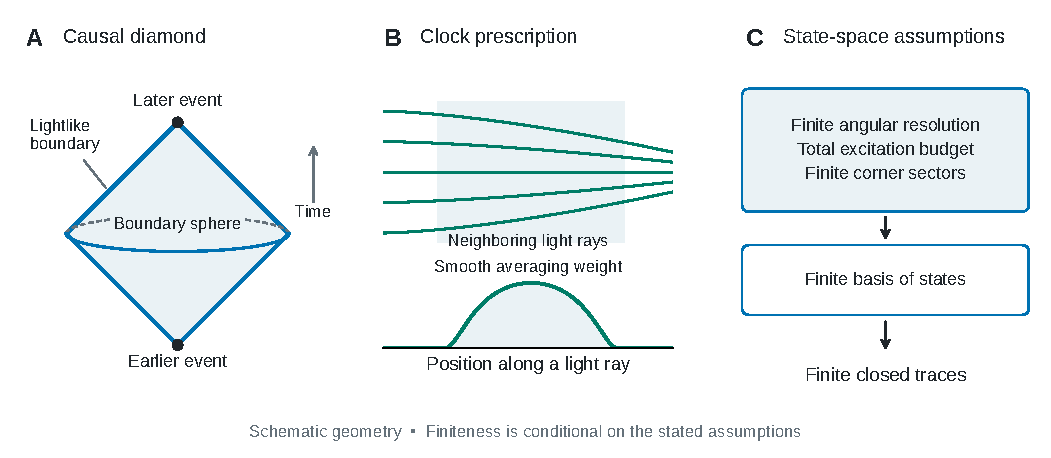
\includegraphics[width=\textwidth]{figs/review_01_causal_diamond.pdf}
\caption{\textbf{From a region bounded by light to a finite model.} (A) The causal diamond contains events that can receive a signal from the earlier tip and send one to the later tip. The ellipse represents a spherical cross-section. (B) Neighboring light rays focus; the modified clock subtracts the vacuum contribution and averages over a smooth weight. Ray paths are schematic and the weight is the rescaled taper of Sec.~\ref{sec:unified_clock}. (C) Finite angular resolution, a total excitation budget, and finite corner sectors supply a finite basis. Closed traces are finite as a consequence of these explicit assumptions.}
\label{fig:geometry}
\end{figure*}

\section{The Continuum Gaps and the Changes Made Here}\label{sec:audit}

\subsection{What the original construction supplies}\label{sec:audit_pass}

The classical proposal describes general relativity using characteristic null data, boundary degrees of freedom, and boundary terms~\cite{Chandrasekaran2026}. Our symbolic calculations check selected local identities in its focusing equations and boundary charges. They do not establish global regularity, the domains of inverse operators, or a complete quantum dynamics. The proposal also gives a conditional correspondence between Lorentzian and Euclidean descriptions of gluing. One of its assumptions is that specified closed contractions are finite. Such a conditional correspondence is useful, but does not independently prove that gravity satisfies this finiteness assumption.

\subsection{Closed amplitudes need an independent convergence argument}\label{sec:audit_fail}

An open amplitude has fixed initial and final states, such as $\langle\phi|U|\psi\rangle$. A closed trace instead sums diagonal amplitudes over a complete basis. Cauchy--Schwarz control of the first expression does not establish convergence of the second. For a positive operator $A\ge c\mathbf{1}$ with $c>0$,
\begin{equation}\label{eq:trace_gap}
\Tr A<\infty\quad\Longrightarrow\quad
\dim\calH\le \frac{\Tr A}{c}<\infty.
\end{equation}
Thus, assuming finite closed-trace convergence at this step would already supply the desired conclusion. The original finite-diamond argument needs an independent reason that its closed-cut partial sums converge to the uncut amplitude; its thermal argument likewise needs convergence over arbitrary finite subsets of the joint cut. The open-amplitude estimates do not supply either implication.

Our response is to change the state space explicitly. A total excitation budget and finite corner sectors give finitely many basis states. All ordinary matrix traces are then finite, without rearranging an infinite signed sum. This establishes trace control for the modified finite model; it does not prove that the original continuum clock enforces the same state space.

\subsection{The clock needs short-distance control and a new lower bound}\label{sec:audit_clock}

The focusing clock contains products of quantum fields at coincident points. In its quadratic oscillator approximation, the un-subtracted vacuum contribution grows with the number of retained modes. The original fixed-resolution estimates do not establish a cutoff-uniform dense domain for the full nonlinear clock. Its limiting-form construction permits a proper domain subspace, so nontriviality must be demonstrated rather than inferred from the finite-mode calculation. Conversely, these observations alone do not prove that the exact gravitational Hilbert space is empty.

We subtract the vacuum contribution and average with a smooth function supported inside the null interval. Subtraction removes the manifest vacuum term but permits negative renormalized focusing: classical positivity can no longer be used unchanged. The quadratic-mode calculation instead uses an independently derived oscillator lower bound and projected second-moment estimates (Sec.~\ref{sec:unified_clock}). Their extension to the complete constrained nonlinear operator remains open. The original paper already uses local vacuum subtraction in a separate semiclassical calculation; the issue here is establishing consistent operator control for its nonperturbative clock.

\subsection{Finite angular resolution alone does not give finite state count}

Replacing a sphere by matrices limits angular modes, but each remaining bosonic mode can still contain arbitrarily many quanta; radial frequencies also remain unbounded without another restriction. We therefore impose a total cost, $\sum n_{k,j,m,p}(k+t_j^2/k)\le B$, in addition to the angular cutoff and finite corner sectors. The cost penalizes radial frequency, angular structure, and occupation number together. Section~\ref{sec:unified_H} gives the counting argument and an exactly enumerable 31-state example.

The original selected-angular-sector Gaussian amplitude, perturbative radiative state count, and conditional algebraic reconstruction motivate comparisons, but none replaces this missing dynamical derivation. A pure-state representation also does not determine every area-changing amplitude from the fixed-area data. We keep those questions open. Table~\ref{tab:changes} states what each modification does and what it does not establish.

\begin{table*}[t]
\caption{From the continuum concerns to explicit assumptions in the finite model. Each row distinguishes a controlled model statement from an outstanding gravitational derivation.}
\label{tab:changes}
\begin{ruledtabular}
\begin{tabular}{p{0.21\textwidth}p{0.35\textwidth}p{0.35\textwidth}}
Issue & Change made here & Scope of the result \\
\colrule
Closed state sums & Count a budget-limited state space with finite corner sectors before taking traces & Finite traces at fixed model parameters; the gravitational origin of the restriction remains open \\
Short-distance clock fluctuations & Vacuum subtraction and smooth averaging; use replacement lower bounds & Controlled quadratic-mode estimates; a nonlinear continuum clock is not constructed \\
Unbounded mode occupations & Bound the total radial, angular, and occupation cost & Finite radiative sector; angular resolution alone would not suffice \\
Removing the regulators & Display cutoff dependence and test selected benchmarks & Consistency evidence at finite resolution; no ultraviolet completion or unified continuum limit is established \\
\end{tabular}
\end{ruledtabular}
\end{table*}

\section{Finite Angular Models and the Clock Restriction}\label{sec:unified}

We represent the null-cone fields on a fuzzy sphere whose matrix rank is tied to the corner area, use a smoothly averaged clock in the mode approximation, and impose an area-scaled occupation budget. The finite-state conclusion below is conditional on these choices.

\subsection{Fuzzy Monopole Bundles, Matrix Vertices, and the Bulk Action}\label{sec:unified_action}

At corner dimensionless area $s=\scrA/(4G_N\hbar)=M s_{\min}$ built from elementary area quanta (embadons), we set the fuzzy-sphere rank to $N=J_{\max}(s)+1\le\lfloor\sqrt{s/s_{\min}}\rfloor+1$. Rather than embedding gravity inside a Yang--Mills matrix model, in which covariant quantum-spacetime backgrounds also carry higher-spin towers~\cite{Steinacker2026}, we represent each Bondi--Sachs field of spin weight $s_w\in\{0,\pm 1,\pm 2\}$ directly as a rectangular matrix in the $SU(2)$-equivariant fuzzy monopole bundle
\begin{equation}\label{eq:fuzzy_bundle}
\calB_{s_w}^{(N)} \;=\; \mathrm{Hom}\!\left(V_{\frac{N-1-s_w}{2}},\, V_{\frac{N-1+s_w}{2}}\right) \;\cong\; \bigoplus_{j=|s_w|}^{N-1} V_j,
\end{equation}
of dimension $\dim\calB_{s_w}^{(N)}=(N+s_w)(N-s_w)=N^2-s_w^2$. Scalars ($\widehat{\rho}^2,\widehat{N},\widehat{F}\in\calB_0^{(N)}$) are $N\times N$ Hermitian matrices ($j=0\dots N-1$); complex shift and H\'aji\v{c}ek one-forms ($\widehat{V},\widehat{w}\in\calB_{+1}^{(N)}$) are $(N+1)\times(N-1)$ matrices ($j=1\dots N-1$); and spin-2 shear data ($\widehat{Z}\in\calB_{+2}^{(N)}$) are $(N+2)\times(N-2)$ matrices ($j=2\dots N-1$). By construction, $\calB_{s_w}^{(N)}$ carries no spurious $j<|s_w|$ modes and no $|s_w|>2$ fields.

The $SU(2)$-intertwining fuzzy Newman--Penrose ladder operators $\widehat{\ethop}:\calB_{s_w}^{(N)}\to\calB_{s_w+1}^{(N)}$ and $\widehat{\bareth}:\calB_{s_w}^{(N)}\to\calB_{s_w-1}^{(N)}$ satisfy
\begin{align}\label{eq:fuzzy_eth}
[\widehat{\bareth},\widehat{\ethop}] &= 2 s_w\,\mathrm{Id}, \nonumber\\
-\widehat{\ethop}\widehat{\bareth}\big|_{\calB_2^{(N)}} &= L^2 - 2 = (j-1)(j+2) = 2 t_j^2,
\end{align}
preserving the round-sphere curvature $R[S^2]=+2$ at every finite $N\ge 3$.

To specify a finite matrix interaction inspired by Appendix~B of Ref.~\cite{Chandrasekaran2026}, we must specify how an $N\times N$ scalar $F\in\calB_0^{(N)}$ contracts with rectangular products such as $Z^\dagger Z\in\mathrm{End}(\mathbb{C}^{N-2})$ and $Z Z^\dagger\in\mathrm{End}(\mathbb{C}^{N+2})$ for $Z\in\calB_{+2}^{(N)}$. Let $\{T^{(0,M)}_{j,m}\}_{j=0}^{M-1}$ be the canonical orthonormal fuzzy spherical harmonic basis of $\mathrm{End}(\mathbb{C}^M)$, normalized by $\frac{1}{M}\Tr_M(T^{(0,M)\dagger}_{j,m}T^{(0,M)}_{j',m'})=\delta_{jj'}\delta_{mm'}$. We define the $SU(2)$-equivariant coefficient-transfer map, isometric on the common harmonic subspace, $\iota_{N\to M}:\mathrm{End}(\mathbb{C}^N)\to\mathrm{End}(\mathbb{C}^M)$ by
\begin{align}\label{eq:iota_map}
\iota_{N\to M}(F) := \sum_{j=0}^{\min(N,M)-1}\sum_{m=-j}^{j}\!&\left(\frac{1}{N}\Tr_N\!\big[T^{(0,N)\dagger}_{j,m}\,F\big]\right) \nonumber\\
&\times T^{(0,M)}_{j,m}.
\end{align}
With Eq.~\eqref{eq:iota_map}, the parity-symmetrized cubic interaction corresponding to $\int_{S^2} F\,Z_2^* Z_3\,\frac{d\Omega}{4\pi}$ is completely specified in matrix form as
\begin{align}\label{eq:cubic_vertex}
\mathcal{V}_3^{(N)}[F;Z_2,Z_3]
&:= \frac{1}{2\sqrt{N^2-4}}\Big[\Tr_{N-2}\!\big(\iota_{N\to N-2}(F)\,Z_2^\dagger Z_3\big) \nonumber\\
&\quad + \Tr_{N+2}\!\big(\iota_{N\to N+2}(F)\,Z_3 Z_2^\dagger\big)\Big] \nonumber\\
&= \frac{1}{N}\Tr_N\!\big(F\,\mathcal{S}_N^{(2)}(Z_2^\dagger,Z_3)\big),
\end{align}
where $\mathcal{S}_N^{(2)}(Z_2^\dagger,Z_3)=\frac{1}{2\sqrt{N^2-4}}[(N-2)\iota_{N-2\to N}(Z_2^\dagger Z_3)+(N+2)\iota_{N+2\to N}(Z_3 Z_2^\dagger)]\in\calB_0^{(N)}$. Evaluating Eq.~\eqref{eq:cubic_vertex} on basis harmonics $T^{(0,N)}_{j_1 m_1}$ and $T^{(+2,N)}_{j_2 m_2},T^{(+2,N)}_{j_3 m_3}$ gives the closed-form Wigner-$6j$ cubic vertex (with $j_L=\frac{N+1}{2}$ and $j_R=\frac{N-3}{2}$):
\begin{align}\label{eq:wigner6j}
&|C^{(N)}_{j_1 m_1;j_2 m_2;j_3 m_3}|
= \frac{1}{2}\sqrt{(2j_1+1)(2j_2+1)(2j_3+1)} \nonumber\\
&\quad\times \left|\begin{pmatrix}j_1&j_2&j_3\\m_1&-m_2&m_3\end{pmatrix}\right|
\Bigg|\sqrt{N-2}\begin{Bmatrix}j_1&j_2&j_3\\j_L&j_R&j_R\end{Bmatrix} \nonumber\\
&\qquad + (-1)^{j_1+j_2+j_3}\sqrt{N+2}\begin{Bmatrix}j_1&j_2&j_3\\j_R&j_L&j_L\end{Bmatrix}\Bigg|.
\end{align}
Direct matrix evaluation confirms both the adjoint relation~\eqref{eq:cubic_vertex} and Eq.~\eqref{eq:wigner6j} to machine precision ($\sim 10^{-14}$), along with exact $SU(2)$ invariance. Parity symmetrization cancels the $O(1/N)$ shift present in one-sided traces $\Tr_{N-2}(\iota(F)Z^\dagger Z)$ ($p=1.06$), yielding $O(1/N^2)$ convergence to the continuum spin-weighted Gaunt integral ($p=2.05$ for $(2,2,2)$), as shown in Fig.~\ref{fig:v2}(A).

Appendix~\ref{app:explicit_action} replaces the former action, which fails its spherical variational test, with a definite nonlinear Einstein--Hilbert angular Galerkin bulk action $I_{\mathrm{G},N}^{\mathrm{bulk}}$. In this prescription finite matrices encode harmonic coefficients; nonlinear products are taken after reconstructing the metric. All ten metric components are varied before gauge fixing. Schwarzschild--de Sitter is then a stationary background, including the mass-conservation equation omitted by premature null gauge fixing. The retained Einstein quadratic sectors follow from this pullback construction. On an exact nonspherical stationary solution, some retained temporal constraints have nonzero Poisson brackets even when all constraints vanish (Proposition~\ref{prop:oblate_rank}). This replacement is not a derivation of Eq.~\eqref{eq:cubic_vertex} or of the simulated Euclidean action.

The archived Kerr and wave calculations in Fig.~\ref{fig:unified}(A) test selected matrix-product contractions, with approximate $N^{-2}$ convergence. They are not variations of a nonlinear gravitational action. The discrete corner spectrum and the relation between the reconstructed bulk action, the projected Hamiltonian examples, and the sampled model remain independent assumptions or open derivations.

\subsection{A Uniform Oscillator Bound and the Occupation-Projected Clock}\label{sec:unified_clock}

To study the clock-domain issue in Sec.~\ref{sec:audit_clock}, we specify a quadratic oscillator model smeared with
$g(u)=\exp[1-(4u(1-u))^{-1}]$ for $0<u<1$, extended smoothly by zero.
Set $c_n=\int_0^1g(u)^2\cos(2\pi n u)\,du$ and $\mu_j=t_j/(2\pi)$.
The positive Gram matrices $M_q,M_p$ defined in Appendix~\ref{app:clock_proof} give
\begin{equation}\label{eq:oscillator_clock}
H_\mu^{\mathrm{NO}}=\tfrac12(q^TM_q q+p^TM_p p)
-\tfrac14\Tr(M_q+M_p).
\end{equation}
The scalar-field bounds of Flanagan and Fewster--Eveson~\cite{Flanagan1997,FewsterEveson1998} are relevant context, but do not supply the previously claimed floor for this canonical clock. We replace that attribution with an explicit bound for Eq.~\eqref{eq:oscillator_clock}:
\begin{equation}\label{eq:clock_floor}
H_\mu^{\mathrm{NO}}\ge-K_g\mathbf1,\qquad
K_g=\frac12\sum_{n=1}^{\infty}(2n^2-n)|c_n|<\infty.
\end{equation}
The proof uses the Powers--St\o rmer trace inequality~\cite{PowersStormer1970} and a bound on the pair kernel $K_\mu=(M_q-M_p)/2$. It is uniform in both $\mu\ge0$ and the radial truncation. It does not construct the full nonlinear gravitational clock. Fourier coefficients through $n=80$, with an analytic fourth-derivative tail bound evaluated by numerical quadrature, give a conservative estimate $K_g\lesssim0.61564$. The analytic expression is the bound; the decimal is not an interval certificate.

The observable must use the total occupation projector $P_B$ of Eq.~\eqref{eq:cross_focusing}. With $d_j=2(2j+1)$, define
\begin{align}\label{eq:compressed_clock}
\Xi_s&=\frac1s\sum_{j=2}^{J(s)}\sum_{m,p}H_{\mu_j}^{\mathrm{NO}},\nonumber\\
\Xi_{s,B}&=\left.P_B\Xi_sP_B\right|_{\operatorname{ran}P_B},\qquad
\tau_{s,B}=u_{\mathrm{cl}}(s)e^{\Xi_{s,B}}.
\end{align}
Every matrix element of the compression is fixed once the radial truncation includes all $k\le B$. In general $e^{P_B\Xi_sP_B}$ on $\operatorname{ran}P_B$ differs from $P_Be^{\Xi_s}P_B$. Radial-mode truncation alone leaves occupation unrestricted. Gaussian determinant methods~\cite{BalianBrezin1969} and stress-tensor tail studies~\cite{FewsterFordRoman2010} therefore cannot be used to identify the former observable with the latter. The earlier large-area exponential moments and Chernoff estimates are withdrawn for the occupation-projected clock.

For $\eta=\ln(\ell/u_{\mathrm{cl}})>0$, spectral calculus gives
\begin{equation}\label{eq:clock_proj_equiv}
P_{\ell,s}=\mathbf1_{(-\infty,\ell]}(\tau_{s,B})
=\mathbf1_{(-\infty,\eta]}(\Xi_{s,B}).
\end{equation}
The normal-ordered vacuum has zero mean. Its second moment requires only the allowed pair states:
\begin{align}\label{eq:projected_clock_variance}
v_{s,B}&=\frac1{2s^2}\sum_{j=2}^{J(s)}d_j\sum_{k,l\ge1}
|(K_{\mu_j})_{kl}|^2\,
\mathbf1_{\omega_{k,j}+\omega_{l,j}\le B},\nonumber\\
\langle0|P_{\ell,s}|0\rangle&\ge1-\frac{v_{s,B}}{\eta^2}.
\end{align}
Here the budget cost $\omega_{k,j}=k+t_j^2/k$ is distinct from the oscillator frequency $\sqrt{k^2+\mu_j^2}$. For $Q_*=1/2$, $s=5000$, $B=2500$, and $J(s)=\lfloor\sqrt{s/\ln3}\rfloor=67$, the computed variance is $5.2467912\times10^{-7}$. At $\ell/u_{\mathrm{cl}}=2$ this gives vacuum acceptance at least $0.9999989079$ [Fig.~\ref{fig:v2}(D)]. This is a spectral probability bound for the vacuum, not a sampling acceptance rate or an all-state estimate. Doubling the Fourier grid changes the variance by about $10^{-22}$; this checks quadrature, not the modeling assumptions.

For $B<12$, no four-particle state is allowed, so the vacuum spectral measure can be computed exactly in the vacuum-plus-pair sector. At $B=4$ the vacuum has no allowed pair partner and $\langle e^{\Xi_{s,B}}\rangle_0=1$ exactly. At $(s,B)=(12,6)$ and $(20,10)$, the means are $1.0000629275$ and $1.0000505663$, and the variances of $e^{\Xi_{s,B}}$ are $1.4563867\times10^{-4}$ and $1.0583928\times10^{-4}$, respectively. These values do not define a monotone law as new states enter the budget.

\begin{proposition}[Conditional finite-area and finite-state bound]\label{prop:finite_area}
Assume $s_M=M s_{\min}>0$ with finite corner degeneracy at each integer $M$, $u_{\mathrm{cl}}(s)=c_0\sqrt{s}$ with $c_0>0$, $J(s)\le\lfloor\sqrt{s/s_{\min}}\rfloor$, and the occupation budget $B(s)=sQ_*$ with fixed $Q_*>0$. Then the clock restriction $\tau_{s,B}\le\ell$ admits only finitely many area sectors, each with finitely many states.
\end{proposition}
\begin{proof}
For $J\ge2$, the number of independent real oscillator channels is $D(J)=2[(J+1)^2-4]$ and
$D(J)/J^2\le8/3$. Thus $\Xi_{s,B}\ge-C_g\mathbf1$ with $C_g=8K_g/(3s_{\min})$; for $J<2$ the sum is empty. Spectral calculus gives
\begin{equation}\label{eq:finite_area_clock}
\tau_{s,B}\ge c_0\sqrt{s}\,e^{-C_g}\mathbf1,
\qquad s\le(\ell/c_0)^2e^{2C_g}
\end{equation}
whenever the clock projector is nonzero. Only finitely many $M$ satisfy this inequality. Equation~\eqref{eq:cross_focusing} bounds the number of modes and every occupation in each sector, proving the claim.
\end{proof}
The conservative expression for $e^{2C_g}$ evaluates to approximately $19.86$ at $s_{\min}=\ln3$; it does not support the previous $1.0036$ precision claim. Also,
$v_{s,B}\le2D(J)K_g^2/s^2\le16K_g^2/(3s_{\min}s)$, giving a uniform $O(1/s)$ vacuum rejection bound for fixed positive $\eta$. This theorem strengthens the model's finiteness result while keeping the clock normalization, angular rule, spectrum, and budget explicit assumptions.


\subsection{Area-Scaled Budget $B(s)=s Q_*$, Projected Dynamics $H_{\mathrm{phys}}$, and Type~I Gluing}\label{sec:unified_H}

The radial focusing clock alone does not explicitly penalize fine angular structure. Classical focusing and transverse-curvature constraints motivate combining a radial allowance $Q_R$ with a transverse allowance $Q_\perp$. We set $Q_*:=Q_R+Q_\perp>0$ and impose the following quantum occupation budget at fixed dimensionless corner area $s=\scrA/(4G_N\hbar)$. This is an additional model assumption, not a consequence proved for the original nonlinear clock:
\begin{align}\label{eq:cross_focusing}
\sum_{k,j,m,p} n_{k,j,m,p}\,\omega_{k,j} &\;\le\; B(s) := s Q_*, \nonumber\\
\omega_{k,j} &= k + \frac{t_j^2}{k} \;\ge\; \max(k,2t_j),
\end{align}
with $t_j^2=\frac{1}{2}(j-1)(j+2)$. Because $\omega_{k,j}\ge 1$ and $\omega_{k,j}\ge\max(k,2t_j)$, Eq.~\eqref{eq:cross_focusing} bounds both the active mode set ($k\le B(s)$, $j\le B(s)/\sqrt{2}$) and every occupation number ($n_{k,j,m,p}\le B(s)$) without circularity. Summing exact integer-partition counts across spin-$\frac{1}{2}$-plus-vacuum corner sectors $M\in\{2,4,6,8,10,15,20\}$ ($s_M=M\ln 3$, $B=6$) yields $\dim\calH=7.726\times 10^{11}$ and a finite Axiom~5 trace $Z_{\scrD,1}=\Tr_{\calH}(e^{-\hat{s}})=1311.33$.

For a directly enumerable example, $B=4$ admits 30 one-graviton states and the vacuum, yielding $\dim\calH_{\mathrm{rad}}=31$ at fixed corner data (Fig.~\ref{fig:state_count}).
\begin{figure*}[t]
\centering
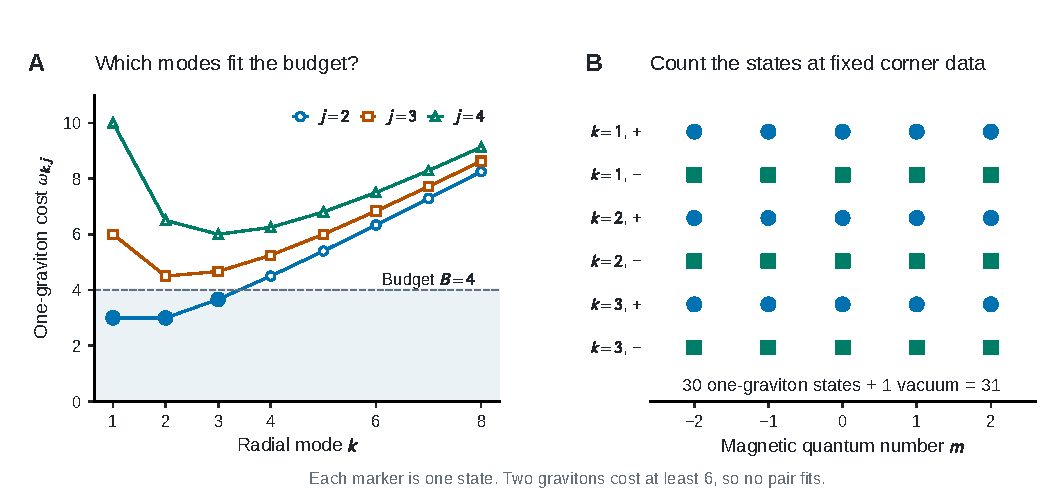
\includegraphics[width=\textwidth]{figs/review_02_state_count.pdf}
\caption{\textbf{An exactly enumerable 31-state radiative sector.} (A) Discrete costs $\omega_{k,j}=k+(j-1)(j+2)/(2k)$ for three angular modes. Filled markers lie within the total budget $B=4$; only $(j,k)=(2,1),(2,2),(2,3)$ qualify, with costs $3,3,11/3$. Lines connect discrete values as guides. (B) Each marker is one one-graviton basis state: three radial modes, five magnetic substates, and two polarization labels ($+$ and $-$). The vacuum adds one state. Every two-graviton state costs at least six. The count fixes the corner sector and assumes $J_{\max}\ge2$.}
\label{fig:state_count}
\end{figure*}

As a separate finite interacting model, define a Hamiltonian that preserves the budget sector via the projector $P_{B(s)}$ as
\begin{equation}\label{eq:H_phys}
H_{\mathrm{phys}} := P_{B(s)}\,H_{\mathrm{model}}\,P_{B(s)}, \qquad H_{\mathrm{model}} = H_0 + \widehat{\mathcal{V}}_3^{(N)},
\end{equation}
This is not asserted to be the canonical Hamiltonian of $I_{\mathrm{G},N}^{\mathrm{bulk}}$. Here $\widehat{\mathcal{V}}_3^{(N)}$ is constructed directly from the Wigner-$6j$ cubic vertex~\eqref{eq:cubic_vertex}--\eqref{eq:wigner6j}. By idempotence $P_{B(s)}^2=P_{B(s)}$, unitary evolution $U_t=e^{-it H_{\mathrm{phys}}}$ leaves $P_{B(s)}\calH$ strictly invariant: $\|(1-P_B)U_t P_B\|=0$. Evaluating Eq.~\eqref{eq:H_phys} on an 88-state $1\leftrightarrow 2$ graviton-focusing Fock space projected to its 19-state physical sector ($B=9$) across $N=6\dots 32$ confirms zero leakage and $O(1/N^2)$ convergence of both the interacting $1\to 2$ transition probability ($p=2.03$) and the projected one-loop graviton self-energy ($p=2.02$) to the corresponding continuum-vertex calculation [Fig.~\ref{fig:v2}(B)].

Replacing infinite-dimensional $\mathrm{Diff}(S^2)$~\cite{CiambelliKlinger2026} by compact $SU(2)$ corner rotations on $\calH_{\scrD}^{\mathrm{FSG}}=\bigoplus_{M\in\{2,4,6\}}\calH_{\mathrm{corner}}(M)\otimes\calH_{\mathrm{rad}}^{\mathrm{RW+Z}}(M)$ ($\dim_{\mathrm{rad}}=15$; explicit operator formula in Appendix~\ref{app:explicit_action}) using spin-$\frac{1}{2}$ embadons ($s_M=M\ln 2$, $\dim\calH_{\mathrm{corner}}(M)=2^M$) gives sector dimensions $(d_2,d_4,d_6)=(60,240,960)$ ($\dim\calH_{\scrD}^{\mathrm{FSG}}=1{,}260$) and Boltzmann weights $(e^{-s_2},e^{-s_4},e^{-s_6})=(\frac{1}{4},\frac{1}{16},\frac{1}{64})$. The resulting Axiom~5 trace is $Z_{\scrD,1}=60/4+240/16+960/64=45.0000$. (With the $s_M=M\ln 3$ spectrum instead, $729 Z=81 d_2+9 d_4+d_6\equiv 4\pmod 8$ for any integers $d_2+d_4+d_6=1260$, whereas $729\times 45\equiv 5\pmod 8$, so $Z_{\scrD,1}=45$ uniquely reflects the $M\ln 2$ spectrum.) On this 1,260-state space, $H_{\mathrm{glue}}$ is $SU(2)$-invariant ($\max_i\|[H_{\mathrm{glue}},J_i]\|=3.09\times 10^{-14}$), has a bounded positive inverse lapse $\widehat{N}^{-1}\in[0.9998,30.7195]$, generates a unique unitary area-changing gluing operator $U_{\calM}$ (singlet transitions $|\langle 4|U|2\rangle|=0.22285$, $|\langle 6|U|4\rangle|=0.22281$), admits reflection-positive $K_{\calM}$ ($\lambda_{\min}=4.385\times 10^{-2}>0$, $Z_{\mathrm{Euc}}=13.9026$), and satisfies the corresponding finite-matrix Lorentzian--Euclidean contraction identity.



\subsection{Regge--Wheeler/Zerilli Perturbations, Boost Closure, and Caustic Bounce}\label{sec:unified_rw}

Constraint elimination in the Einstein quadratic action, now derived symbolically and represented in the finite bundles as Eq.~\eqref{eq:quadratic_matrix_action}, gives the axial constraint $\partial_t h_0=f\partial_r(f h_1)$ and the Regge--Wheeler potential $V_{\mathrm{RW}}^{(j)}(r)=f(r)[j(j+1)/r^2-6M/r^3]$, together with the general-$j$ Chandrasekhar--Darboux intertwining identity $V_{\mathrm{RW/Z}}=W^2\mp dW/dr_*+\beta$ for $W(r)=3Mf/[r(\lambda r+3M)]+\lambda(\lambda+1)/(3M)$ ($\lambda=t_j^2$). Fourth-order Numerov scattering integration across $j=2\dots 8$ verifies Chandrasekhar isospectrality ($||T_{\mathrm{RW}}|^2-|T_{\mathrm{Z}}|^2|$ down to $2.86\times 10^{-6}$); the paramagnetic $-6M/r^3$ Weyl tidal term lowers the $j=2$ barrier by $-38.8\%$ ($0.15128$ versus $0.24711$) and boosts peak transmission by a factor of $16.3$ [Fig.~\ref{fig:unified}(B)].

Because noncompact $SO(3,1)$ has no faithful finite-dimensional unitary representation, we examine truncated Gel'fand--Naimark spin-2 generators $(L_i^{(N)},K_i^{(N)})$ on $\calB_2^{(N)}$. Direct evaluation across $N=6\dots 24$ confirms exact $[L,L]$ and $[L,K]$ commutation everywhere, exact boost closure $([K_i,K_j]+i\epsilon_{ijk}L_k)|j,m\rangle=0$, and exact Lorentz Casimirs ($C_1=+2,C_2=-2$) on every mode $j\le N-2$, confining the entire boost defect to the single Planckian shell $j=N-1$. Finite-rapidity boosts of a localized $j=2$ wavepacket recover continuum $SO(3,1)$ exponentially in $N$, with infidelity reaching $1.55\times 10^{-15}$ by $N=18$ ($\eta=0.5$), $2.66\times 10^{-15}$ by $N=32$ ($\eta=1.0$), and $1.33\times 10^{-12}$ by $N=44$ ($\eta=1.5$) [Fig.~\ref{fig:unified}(C)]. Under strong shear focusing ($\sigma_0=3.0$, classical caustic $\rho\to 0$ at $v_c=0.7405$), the minimal embadon area barrier ($s_{\min}=\ln 3$) is modeled by the Ermakov--Pinney trajectory $\rho_Q(v)=\sqrt{r_0^2\cos^2(\omega v)+\rho_{\min}^2\sin^2(\omega v)}$ that matches classical general relativity to $0.036\%$ in the semiclassical regime and bounces smoothly at $\rho_{\min}=\sqrt{\ln 3/\pi}\,\lP=0.5914\,\lP$ [Fig.~\ref{fig:unified}(D)].

\section{Monte Carlo of the Euclidean Matrix Model}\label{sec:hmc}

We study nonperturbative sampling of a finite Euclidean matrix model motivated by the preceding vertex construction. A derivation equating its measure and dynamics to the complete constrained Lorentzian action is still required. The sampled path integral is
\begin{equation}\label{eq:hmc_Z}
Z^{(N)} = \int \mathcal{D}\Phi\,\mathcal{D}_{\widehat{\rho}} Z\,\mathcal{D}_{\widehat{\rho}} Z^\dagger\,\exp\!\big(-S_E^{(N)}[\Phi,Z]\big)
\end{equation}
on a periodic radial-time lattice $T^2$ ($N_\tau\times N_r$) fibered with the fuzzy monopole bundles $\Phi(x)\in\calB_0^{(N)}$ ($N\times N$ Hermitian, representing the conformal area fluctuation $\widehat{\rho}^2/r_0^2=\exp(g_N\Phi)$) and $Z(x)\in\calB_{+2}^{(N)}$ ($(N+2)\times(N-2)$ complex spin-2 shear).

Using the parity-symmetrized embedding $\iota_{N\to N\pm s}$ of Eq.~\eqref{eq:iota_map} and the exact $SU(2)$-intertwining spin-lowering map $\widehat{\bareth}:\calB_{+2}^{(N)}\to\calB_{+1}^{(N)}$ satisfying $\langle\widehat{\bareth}Z,\widehat{\bareth}Z\rangle_{1,N}=\langle Z,(L^2-2)Z\rangle_{2,N}$, where $\langle U,V\rangle_{s,N}=\Tr(U^\dagger V)/\sqrt{N^2-s^2}$, the Euclidean action, with a nonnegative shear contribution, is
\begin{align}\label{eq:hmc_action}
&S_E^{(N)} = \sum_{x\in T^2}\Bigg\{\frac{1}{2}\Tr_N\!\Big[(\nabla_\parallel\Phi)^2 + \Phi L^2\Phi + \mu^2\Phi^2 + \tfrac{\lambda_4}{2N}\Phi^4\Big] \nonumber\\
&\quad + \frac{1}{2}\Big[\Tr_{N-2}\!\big(e^{g_N\iota_{N\to N-2}(\Phi)}|\nabla_\parallel Z|_R^2\big) \nonumber\\
&\qquad + \Tr_{N+2}\!\big(e^{g_N\iota_{N\to N+2}(\Phi)}|\nabla_\parallel Z|_L^2\big)\Big] \nonumber\\
&\quad + \frac{1}{2}\Big[\Tr_{N-1}\!\big(e^{g_N\iota_{N\to N-1}(\Phi)}(\widehat{\bareth}Z)^\dagger\widehat{\bareth}Z\big) \nonumber\\
&\qquad + \Tr_{N+1}\!\big(e^{g_N\iota_{N\to N+1}(\Phi)}\widehat{\bareth}Z(\widehat{\bareth}Z)^\dagger\big)\Big]\Bigg\} + S_{\mathrm{DW}},
\end{align}
where $|\nabla_\parallel Z|_R^2=(\partial_\tau Z)^\dagger\partial_\tau Z+(\partial_r Z)^\dagger\partial_r Z$, $|\nabla_\parallel Z|_L^2=\partial_\tau Z(\partial_\tau Z)^\dagger+\partial_r Z(\partial_r Z)^\dagger$, and $S_{\mathrm{DW}}$ encodes the invariant DeWitt--Fujikawa spin-2 path-integral measure $\mathcal{D}_{\widehat{\rho}}Z\,\mathcal{D}_{\widehat{\rho}}Z^\dagger$:
\begin{equation}\label{eq:dewitt_measure}
S_{\mathrm{DW}}[\Phi] = -\frac{g_N(N^2-4)}{N}\sum_{x\in T^2}\Tr_N\!\big(\Phi(x)\big).
\end{equation}
Expanding Eq.~\eqref{eq:hmc_action} to $O(g_N)$ reproduces the exact parity-symmetrized Wigner-$6j$ cubic vertex~\eqref{eq:cubic_vertex}--\eqref{eq:wigner6j}, while the exponential coupling preserves strict positivity $S_{\mathrm{shear}}\ge 0$ for all configurations.

\begin{figure*}[t]
\centering
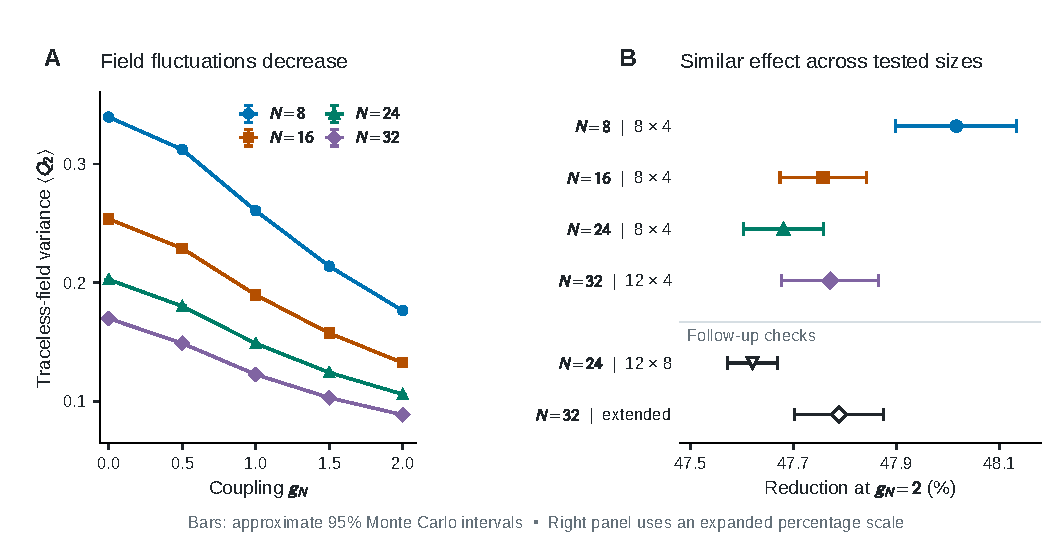
\includegraphics[width=\textwidth]{figs/fig_followup_roughness.pdf}
\caption{\textbf{Coupling suppresses traceless matrix-field fluctuations.} (A) Mean dimensionless traceless matrix-field fluctuation $Q_2$ versus coupling. Colors and shapes identify matrix rank; lines guide the eye. Bars are $1.96$ times the archived Monte Carlo standard error, often smaller than the symbols. (B) Reduction $100[1-\overline Q_2(2)/\overline Q_2(0)]$, using a measured zero-coupling control at the same rank and lattice. The percentage axis is expanded to show size dependence. Bars are the archived approximate 95\% propagated ratio intervals. The four main coupled ensembles use 4--8 chains; the extended $N=32$ check uses 16 chains with 2000 draws per chain, and the $12\times8$ check uses eight with 700. All comparisons retain $\mu^2=0.25$ and $\lambda_4=0.1$. Intervals quantify sampling uncertainty, not model or discretization uncertainty.}
\label{fig:roughness}
\end{figure*}

We sample Eq.~\eqref{eq:hmc_Z} in double precision using Fourier-accelerated hybrid Monte Carlo on $T^2\times S_N^2$. The archived production set contains 28 ensembles with 4--8 chains each. At $N=48$ on a $12\times4$ lattice, each chain contains $N_\tau N_r(3N^2-8)=331{,}392$ real variables. The previously quoted $1{,}325{,}568$ is the sum over four independent replicas.

\paragraph{Matched controls and a larger lattice.}
We define roughness by $Q_2=V^{-1}\sum_x N^{-1}\Tr(\Phi_{\mathrm{trless}}^2)$, the squared norm of the traceless matrix field. With $\mu^2=0.25$ and $\lambda_4=0.1$ held fixed, changing $g_N$ from zero to two reduces its mean by $48.016\%$, $47.758\%$, $47.681\%$, and $47.772\%$ at ranks $8,16,24,32$, respectively [Fig.~\ref{fig:roughness}]. The corresponding approximate 95\% Monte Carlo intervals are $[47.899,48.134]\%$, $[47.674,47.841]\%$, $[47.603,47.758]\%$, and $[47.676,47.866]\%$. The quartic-only change relative to the analytic Gaussian reference is at most $0.17\%$. These matched controls resolve the denominator ambiguity in the earlier Gaussian-baseline comparison. Since the modeled area is the nonlinear matrix exponential $e^{g_N\Phi}$, suppression of $Q_2$ is not by itself a measurement of physical area variance or spacetime smoothing.

At $N=24$, increasing the lattice from $8\times4$ to $12\times8$ gives $47.621\%$ suppression, with interval $[47.572,47.670]\%$. The difference is $-0.060\pm0.047$ percentage points (one standard error; 95\% interval $[-0.151,+0.032]$). This supports persistence over the tested volume change. It does not establish exact rank independence or a continuum extrapolation. The four-rank headline uses archived $g_N=2$ summaries; the extended $N=32$ run provides a full-history cross-check of $47.789\%$.

\paragraph{What convergence and drift mean.}
A Monte Carlo chain is a sequence of correlated sampled configurations. Sampling drift means that estimated distributions or averages continue to change with simulation time. Rank-normalized split-$\hat R$~\cite{Vehtari2021} compares within-chain and between-chain behavior after splitting chains in half; values near one support agreement. Bulk and tail effective sample sizes (ESS) estimate the information available for typical values and distribution tails after accounting for correlations. We use $\hat R<1.01$ and both ESS values at least 400 as diagnostic targets, not proofs of stationarity. This sampling question differs from resolution dependence, the change in a computed quantity when a numerical cutoff or lattice is refined.

A spatially uniform collective move changes $\Phi$ and rescales $Z$ together. The follow-up adds local Fourier-wave moves,
$\Phi(x)\mapsto\Phi(x)+\delta(x)I_N/\sqrt N$ and $Z(x)\mapsto e^{-g_N\delta(x)/(2\sqrt N)}Z(x)$.
The angular shear term is invariant and the measure change cancels the transformation Jacobian. The local move does change the radial-time terms; these enter its Metropolis acceptance probability. Each extended run uses 16 chains with 2000 retained draws per chain.

In these follow-ups, the local mean-area rank-normalized split-$\hat R$ improves from 1.1082 to 1.0098 at fixed-coupling $N=32$, and from 1.0325 to 1.0021 at scaled-coupling $N=48$ [Fig.~\ref{fig:hmc}(B)]. Bulk/tail ESS are 2576/5624 and 4020/9123, respectively. Earlier values 1.416 and 1.181 were ordinary unsplit diagnostics and should not be labeled as the same estimator. The $N=24$, $12\times8$, $g_N=2$ run passes the roughness targets ($\hat R=1.0041$, bulk ESS 896), but its local area remains poorly mixed ($\hat R=1.3268$, bulk ESS 20). Convergence is therefore assessed separately for each observable and ensemble.

\begin{figure*}[t]
\centering
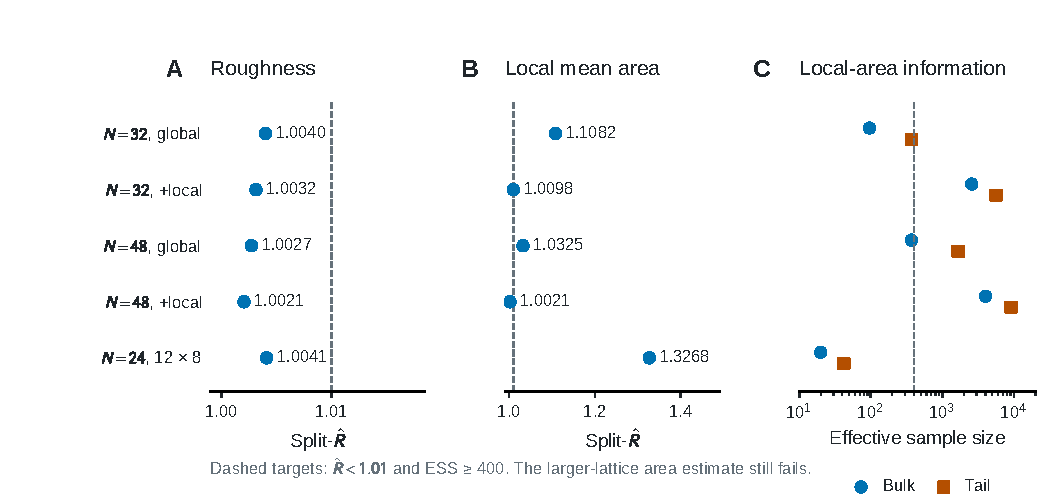
\includegraphics[width=\textwidth]{figs/fig6_modal_b200_hmc.pdf}
\caption{\textbf{Sampling convergence depends on the observable.} Rank-normalized split-$\hat R$ for (A) roughness and (B) local mean area, with different horizontal scales. Values near one indicate agreement across split chains; the target is $\hat R<1.01$. (C) Bulk and tail effective sample sizes (ESS) for local mean area, on a logarithmic axis; the target is at least 400 for each. ``Global'' and ``+local'' identify the successive sampling schemes, with local collective moves added in the latter. The extended $N=32$ and $N=48$ runs use 16 chains with 2000 retained draws per chain; their couplings differ as specified in the text. The $N=24$, $12\times8$ test has eight chains with 700 draws. Its roughness passes the displayed targets while its area remains poorly mixed. These diagnostics do not prove stationarity.}
\label{fig:hmc}
\end{figure*}

\paragraph{Area and spin-2 benchmarks.}
At scaled coupling $g_N=3.3821/\sqrt N$ and $\mu^2=0.05$, the extended $N=48$ run gives local mean area $1.0142\pm0.0009$ (between-chain standard error), with mean extreme eigenvalues $(0.726,1.381)$. At fixed $g_N=2$, $N=32$, these quantities are $1.2107\pm0.0057$ and $(0.342,3.038)$. The matrix $\exp(g_N\Phi)$ is positive by construction for Hermitian $\Phi$. Its positive sampled eigenvalues alone do not prove the absence of physical spacetime caustics.

The archived $N=48$ propagator is close to its free-field value, with fitted wave-function coefficient $Z_{\mathrm{wf}}=1.0008$. The mass-squared fit intercepts at increasing ranks $8,12,16,24,32,48$ are $+0.348,+0.314,+0.137,-0.065,+0.016,+0.077$. Their uncertainties and joint volume/rank extrapolation remain to be established. The Binder statistic of the invariant scalar $Q_2$ alone does not determine spontaneous breaking of $SU(2)$.

\paragraph{Functional measure.}
Earlier $g=2.5$, $\mu^2=0.5$ ensembles show a large area difference with and without the DeWitt term. The ratios of mean areas are approximately 197, 181, and 177 at ranks 8, 16, and 24 on matching lattices. At rank 32 the temporal extents differ. Establishing a phase transition requires matched volumes, observable-specific convergence, and scaling analysis beyond these comparisons.


\section{One-Loop Entropy Benchmarks}\label{sec:1loop}

Purely kinematical embadon horizons reproduce the Bekenstein--Hawking area law $S=s$ with logarithmic coefficient $c_{\log}=0$ (unconstrained compositions, $s_{\min}=\ln 3$) or $c_{\log}=-\frac{3}{2}$ (an $SU(2)$ singlet horizon, matching Kaul and Majumdar~\cite{KaulMajumdar2000}). By contrast, Sen's covariant one-loop computation for four-dimensional pure gravity on Schwarzschild~\cite{Sen2013}, also considered in Ref.~\cite{Chandrasekaran2026}, gives positive coefficients: $+\frac{106}{45}\approx +2.3556$ for mixed angular momentum and $+\frac{77}{90}\approx +0.8556$ in the $J=0$ singlet ensemble.



The covariant benchmarks draw on two complementary methods: on-shell heat-kernel coefficients for perturbative gravity~\cite{BBM2022} and conical-singularity methods for entropy, including extrinsic-curvature terms for general entangling surfaces~\cite{FPS2013}. These references provide methodological context rather than a derivation of the fuzzy-sphere result.

Two results reconcile discrete corners with Sen's positive sign. First, orthonormal-frame evaluation of the four-dimensional de Donder Lichnerowicz operator $\Delta_L h_{ab}=-\nabla^2 h_{ab}-2W_{acbd}h^{cd}$ plus vector ghost on Ricci-flat Schwarzschild splits the Gilkey--Seeley--DeWitt coefficient $a_2$ into three channels:
\begin{align}\label{eq:lich_flip}
\frac{180\,a_2^{\mathrm{GR}}}{K}\Big|_{R_{ab}=0} &= \underbrace{+2}_{\text{2 pol.}} \;\underbrace{-60}_{\Omega_{mn}^2} \;\underbrace{+270}_{\frac{1}{2}\Tr(V^2)} = +212, \nonumber\\
c_{\log}^{\mathrm{bulk}} &= \frac{1}{45}-\frac{2}{3}+3 = +\frac{106}{45}.
\end{align}
Without the paramagnetic spin-2 Weyl tidal term $V_{ab}{}^{cd}=-2W_a{}^c{}_b{}^d$ ($+3\ln s$), bulk gravitons remain negative ($-\frac{29}{45}$). Including dynamical bulk gluing shifts both corner ensembles by $+\frac{106}{45}$, matching both of Sen's predictions simultaneously: $0+\frac{106}{45}=+\frac{106}{45}$ (mixed) and $-\frac{3}{2}+\frac{106}{45}=+\frac{77}{90}$ (singlet).

Second, regulating loops through the dynamical fuzzy sphere $J_{\max}(r)=\sqrt{\pi/s_{\min}}\,r/\lP$ while keeping continuum radial and time directions ($N_{\mathrm{rad}}=\infty$) preserves four-dimensional covariance in every universal logarithmic term.

\begin{theorem}[Four-Dimensional Infrared Isotropy]\label{thm:isotropy}
Let $k_\parallel\in\mathbb{R}^2$ ($x=k_\parallel^2\in[0,A]$) and $k_\perp\in\mathbb{R}^2$ ($y=k_\perp^2\in[0,B]$ with $B=\Lambda_P^2$). Taking the radial-time continuum limit $A\to\infty$ first at fixed transverse cutoff $B$, the infrared logarithmic coefficients $\lim_{m\to 0}(-m\partial_m I)$ of every scalar, rank-2, and rank-4 momentum integral match exact $SO(4)$-isotropic values: $J_0=1$, $(J_\parallel,J_\perp)=(\frac{1}{2},\frac{1}{2})$, and $(K_{\parallel\parallel},K_{\parallel\perp},K_{\perp\perp})=(\frac{1}{3},\frac{1}{6},\frac{1}{3})$.
\end{theorem}

Direct discrete-harmonic integration over curved Euclidean Schwarzschild ($r_H/\lP=10\to 320$, $N_{\mathrm{rad}}=\infty$) is consistent with Theorem~\ref{thm:isotropy}: the asymptotic bulk slope reaches $+2.35334$ ($0.09\%$ from $+\frac{106}{45}$) and the $SU(2)$-singlet total reaches $+0.85334$ ($0.26\%$ from $+\frac{77}{90}$), as shown in Fig.~\ref{fig:1loop}(C)--(D) and Table~\ref{tab:1loop}. On a flat-space $N=200$ radial lattice, regulating $j\ge 2$ gravitons with a smooth Casimir factor $e^{-j(j+1)/(\alpha R_{\mathrm{eff}})^2}$ eliminates the $O(1/\alpha^2)$ Euler--Maclaurin sharp-edge artifact already at $\alpha=2.0$, reproducing Benedetti and Casini's flat-space graviton entanglement entropy $-\frac{61}{45}=-1.35556$~\cite{BenedettiCasini2020} to $0.02\%\text{--}0.12\%$ across $\alpha=2\to 4$ even as the non-universal area term shifts by $+37\%$ [Fig.~\ref{fig:1loop}(B)]. On four-dimensional de Sitter space ($S^4$), combining the high-$n$ transverse-traceless minus vector trace ($+\frac{509}{45}$) with the $n=0,1$ Killing and conformal-Killing edge modes ($-24$) recovers Anninos, Denef, Law, and Sun's $-\frac{571}{45}=-\frac{331}{45}-\frac{16}{3}$~\cite{ADLS2022} [Fig.~\ref{fig:1loop}(D)], while $SO(5)\to SO(4)\to SO(3)$ branching shows $\max j=n$, so every sub-Planckian $S^4$ mode lies inside $S^2_{J_{\max}}$.

\begin{table}[t]
\caption{One-loop logarithmic coefficients ($N_{\mathrm{rad}}=\infty$). Schwarzschild entries use the final radius doubling $160\to320$. The five-radius fits give $2.34557$ and $0.84557$, with errors $0.424\%$ and $1.167\%$.}
\label{tab:1loop}
\begin{ruledtabular}
\begin{tabular}{lccc}
4D Geometry & Covariant & FSG & Err. \\
\colrule
Schw.\ mixed~\cite{Sen2013} & $+\frac{106}{45}$ ($+2.3556$) & $+2.3533$ & $0.09\%$ \\
Schw.\ singlet~\cite{Sen2013} & $+\frac{77}{90}$ ($+0.8556$) & $+0.8533$ & $0.26\%$ \\
Flat EE~\cite{BenedettiCasini2020} & $-\frac{61}{45}$ ($-1.3556$) & $-1.3552$ & $0.02\%$ \\
de Sitter $S^4$~\cite{ADLS2022} & $-\frac{571}{45}$ ($-12.6889$) & $-\frac{571}{45}$ & $0$ \\
\end{tabular}
\end{ruledtabular}
\end{table}

\section{Two-Loop Regulator Analysis, Dynamical Rank Sums, and Sub-Planckian Bounds}\label{sec:uv}

\subsection{Transverse-Only Cutoffs and Fixed-Budget Sums}\label{sec:uv_2loop}

Because Theorem~\ref{thm:isotropy} holds at one loop with a transverse fuzzy-sphere cutoff alone, one might ask whether $S^2_N$ alone regulates higher loops. Power counting and numerical integration over a parallel radial-time cutoff $\Lambda_\parallel/\Lambda_\perp=2\to 32$ show that it does not. Whereas the one-loop $W^2$ integral converges monotonically to $\ln 5=1.60944$ ($1.39813\to 1.60846$), derivative graviton vertices give the two-loop sunset diagram a parallel superficial degree of $+2$, producing a quadratic divergence $I_{\mathrm{2L}}\sim\Lambda_\parallel^2\ln\Lambda_\parallel$ ($1.41\to 4365.05$, fitted slope $p=2.63$) [Fig.~\ref{fig:uv}(A)].

The occupation projector in Eq.~\eqref{eq:cross_focusing} gives a finite-dimensional sector and finite perturbative sums for operators restricted to that sector. A related diagnostic restricts each single-mode label by $\omega_{k,j}\le B$. Its discrete two-loop sum is $251.18$ at $B=4$ (30 modes), $8{,}613.24$ at $B=6$ (138 modes), $67{,}989.28$ at $B=8$ (324 modes), and $372{,}883.33$ at $B=10$ (662 modes), as plotted in Fig.~\ref{fig:budget_growth}. These values apply to the single-mode restriction. A calculation with $P_B$ on every many-particle intermediate state must also enforce its total occupation cost. The rapid growth of the reported diagnostic motivates studying the large-budget limit. The four samples characterize the finite-budget trend, while ultraviolet completeness requires control of the interacting limit $B(s)\to\infty$.


\begin{figure*}[t]
\centering
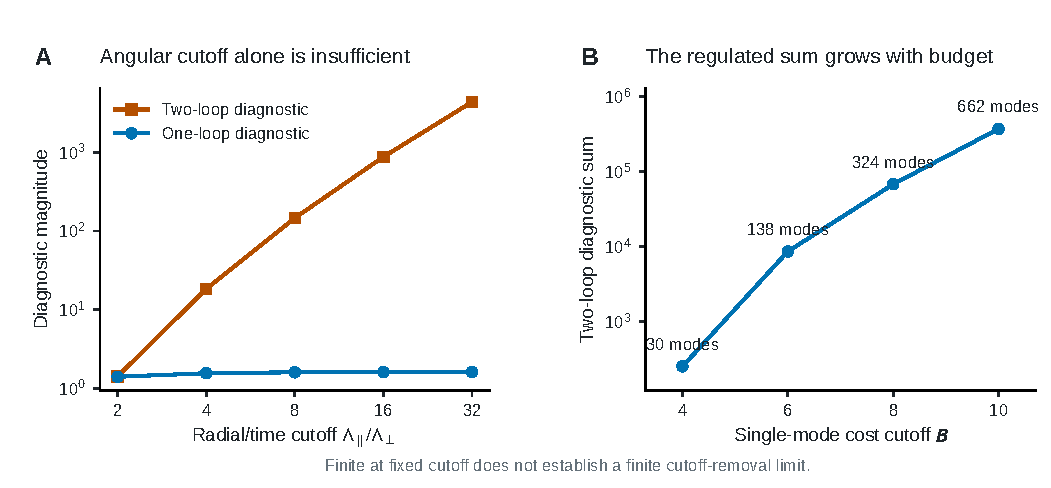
\includegraphics[width=\textwidth]{figs/review_03_two_loop_budget.pdf}
\caption{\textbf{Finite resolution and cutoff removal are different questions.} (A) Archived one- and two-loop diagnostic integrals with fixed angular cutoff as the radial/time cutoff grows. The one-loop expression approaches its reference limit while the two-loop diagnostic grows. (B) The regulated two-loop sum at four single-mode cost cutoffs $\omega_{k,j}\le B$; labels give the admitted mode count. Both vertical axes are logarithmic and lines guide the eye. The many-particle projector also constrains total intermediate-state cost. These fixed-cutoff calculations do not establish a finite ultraviolet limit.}
\label{fig:budget_growth}
\end{figure*}



\subsection{Schwarzschild Goroff--Sagnotti Shift and Sub-Planckian Pixel Bound}\label{sec:uv_cemz}

At two loops in four-dimensional pure gravity, the unique on-shell Goroff--Sagnotti counterterm~\cite{GoroffSagnotti1986} is cubic in the Weyl tensor, $\Delta\mathcal{L}_{\mathrm{GS}}=\frac{209}{2880(4\pi)^4}\kappa^2\ln(\mu/\Lambda_P)\,W_{ab}{}^{cd}W_{cd}{}^{ef}W_{ef}{}^{ab}$. Evaluating this invariant on Euclidean Schwarzschild gives $K=48M^2/r^6$, $W^3=-96M^3/r^9$, and $\int d^4x\sqrt{g}\,W^3=-32\pi^3/(\lP^2 s)$, leading to the two-loop Schwarzschild entropy shift
\begin{equation}\label{eq:gs_entropy}
\Delta S_{\mathrm{2\text{-}loop}}^{\mathrm{GS}}(s) \;=\; \frac{209}{1440}\,\frac{\ln(s/s_{\min})}{s},
\end{equation}
which enters at the same $O(1/s)$ order (up to $\ln s$) as the fuzzy-sphere $O(1/N^2)=O(s_{\min}/s)$ correction (ratio $0.596$ at $s=10^2$, $1.204$ at $s=10^4$, $3.030$ at $s=10^{10}$), with flat-space eikonal advance scale~\cite{CEMZ2016} $b_{\mathrm{adv}}^{\mathrm{GS}}=0.0413\,\lP\ll\lP$.

A simple effective-field-theory naturalness criterion constrains the elementary area quantum $s_{\min}$. In the separate matrix-product vertex model, noncommutative modifications appear at order $O(1/N^2)=O(\rho_{\min}^2/r^2)$, controlled by the minimal embadon pixel radius $\rho_{\min}=\sqrt{s_{\min}/\pi}\,\lP$. Requiring these modifications to remain at or below the Planck length ($\rho_{\min}\le\lP$), so that non-Einsteinian three-graviton interactions do not enter at semiclassical impact parameters where eikonal causality bounds~\cite{CEMZ2016} would demand massive higher-spin particles ($J>2$), yields
\begin{equation}\label{eq:cemz_bound}
s_{\min} \;\le\; \pi \;\approx\; 3.14159.
\end{equation}
Deriving a complete gravitational four-point amplitude, including contact terms and constraints beyond the vertex in Eq.~\eqref{eq:wigner6j}, to fix the exact $1/b^2$ versus $1/b^4$ scattering coefficient remains a natural follow-up test of this bound.

\subsection{Dynamical Rank Sums and the $\mathrm{AdS}_4$ Hawking--Page Transition}\label{sec:uv_hp}

Summing dynamically over all fuzzy-sphere ranks $N=3\dots\infty$ with $s_N=s_{\min}N^2$ clarifies the infrared thermodynamics [Fig.~\ref{fig:uv}(B)--(C)]. In asymptotically flat space ($L_{\mathrm{AdS}}\to\infty$), entropy grows quadratically ($S\propto N^2$) while ADM energy grows linearly ($E\propto N$), driving $\ln W_N$ to $+\infty$ ($+27{,}202$ by $N=160$). This reproduces the Gross--Perry--Yaffe Jeans instability~\cite{GrossPerryYaffe1982} and reflects why a finite clock cutoff $\ell(\scrD)$ is physically needed in flat space.

In $\mathrm{AdS}_4$ of curvature radius $L$, the ADM energy acquires a cubic term $E_N=\frac{1}{2}\sqrt{s_N/\pi}+\frac{1}{2}s_N^{3/2}/(\pi^{3/2}L^2)\propto N^3/L^2$ that dominates the $+N^2$ entropy for every $\beta>0$. The discrete-rank partition function converges cleanly and reproduces the four-dimensional Hawking--Page transition~\cite{HawkingPage1983}, with $T_{\mathrm{HP}}L\to 1/\pi=0.318310$ and specific-heat scaling $C_{\mathrm{peak}}/L^4\to 2.45$ across $L/\lP=10\to 80$. At finite $L/\lP=10$ ($s_{\mathrm{HP}}=314.2$), the one-loop logarithmic term shifts the transition temperature in opposite directions depending on whether bulk graviton gluing is included: the glued mixed ($+\frac{106}{45}\ln s$) and singlet ($+\frac{77}{90}\ln s$) ensembles lower $T_{\mathrm{HP}}L$ to $0.299479$ ($-5.9\%$) and $0.308598$ ($-3.1\%$), whereas kinematical LQG ($-\frac{3}{2}\ln s$) raises it to $0.322495$ ($+1.3\%$).

\subsection{Three-Diamond Corner Fusion and Allowed Window for $s_{\min}$}\label{sec:uv_multidiamond}

To test multi-diamond gluing, we constructed a $2{,}048$-dimensional network of three adjacent causal diamonds ($\scrD_A,\scrD_B,\scrD_C$) joined along shared $SU(2)$-singlet embadon corners and coupled to Schwarzschild Regge--Wheeler gravitons. Corner-fusion pentagon associativity holds to $9.5\times 10^{-17}$ and $SU(2)$ coproduct equivariance holds identically. Across all six overlapping subregions ($A,B,C,AB,BC,AC$), generalized entropy additivity $S_{\mathrm{gen}}(R)=s(\partial R)+S_{\mathrm{bulk}}(R)$ holds to $8.88\times 10^{-16}$. As a consistency check (guaranteed structurally by Lieb--Ruskai for any density operator), all Subadditivity and Strong Subadditivity inequalities hold numerically ($I(A:B)=3.53421$, $I(A:C|B)=1.87086$, $I(A:B|C)=3.53421$, $I(B:C|A)=1.95604$).

Combining coarse-graining of the corner entropy ($s_{\min}=\ln(1+d_0)$ when an empty state is included, or $s_{\min}=\ln d_0$ without one, where $d_0\ge 2$ is the local embadon dimension) with the sub-Planckian bound~\eqref{eq:cemz_bound} restricts admissible models to a finite discrete set: $2\le d_0\le 22$ (or $2\le d_0\le 23$). Large-$d_0$ corners violate the bound ($d_0=100\implies \rho_{\min}=1.21\,\lP$), leaving minimal spin-$\frac{1}{2}$ qubit corners ($d_0=2$, $s_{\min}=\ln 2$ with $\rho_{\min}=0.470\,\lP$ or $s_{\min}=\ln 3$ with $\rho_{\min}=0.591\,\lP$) well inside the sub-Planckian window [Fig.~\ref{fig:uv}(D)].

\section{Pair Amplitudes, Gluing, and Semiclassical Backreaction}\label{sec:orig_sections}

We now examine three distinct tests: a regulated Gaussian pair amplitude, finite-matrix gluing identities, and semiclassical backreaction benchmarks. Each calculation is specified below without requiring the original paper. These tests address selected ingredients of the null-cone proposal~\cite{Chandrasekaran2026}; they do not establish equivalence to its complete interacting dynamics.



\subsection{A Budget-Limited Gaussian Pair Amplitude}\label{sec:orig_44}

Summing the four-dimensional graviton modes $(j,m,p,k)$ over $j\in\{2,\dots,J_{\max}(s)\}$ ($J_{\max}=\lfloor\sqrt{s/s_{\min}}\rfloor$) and $k$ satisfying $2\omega_{k,j}=2(k+t_j^2/k)\le B(s)=sQ_*$ of Eq.~\eqref{eq:cross_focusing} defines the following finite Gaussian mode sum at every finite area $s$. It extends the selected-angular-sector example of Ref.~\cite{Chandrasekaran2026} with angular degeneracies and a two-particle budget:
\begin{align}\label{eq:sec44_4d}
\calM_{B(s)}^{\mathrm{FSG}}(s)
&= \sum_{j=2}^{J_{\max}(s)}\frac{2j+1}{s^2}\sum_{2\omega_{k,j}\le B(s)}\frac{e^{-2i(k+t_j^2/k)/s}}{(k+t_j^2/k)^2}.
\end{align}
The factor of two enforces the occupation cost of the intermediate state created by the quadratic insertion. In particular, $B=4$ admits single gravitons but no pair, so $\calM_{B=4}(s)=0$. Set $L=B/2$. An excluded mode obeys $\omega_{k,j}>L$, which implies $k>L/2$ or $k<2t_j^2/L$. Summing the absolute tails gives
\begin{equation}\label{eq:tail_bound}
|\calM_\infty^{\mathrm{FSG}}-\calM_{B(s)}^{\mathrm{FSG}}| = O\!\left(\frac{J_{\max}^2}{s^2 L}+\frac{J_{\max}^4}{s^2 L^3}\right) = O(s^{-2}).
\end{equation}
Here $Q_*>0$ is fixed and $J_{\max}^2=O(s)$. The upper radial tail uses $\omega\ge k$ and $\sum_{k>L/2} k^{-2}=O(L^{-1})$. The lower tail uses $\omega\ge t_j^2/k$ and $\sum_{k<2t_j^2/L} k^2/t_j^4=O(t_j^2/L^3)$. Thus the corrected pair projector preserves the leading real $s^{-3/2}$ term and the imaginary $-\ln s/(s_{\min}s^2)$ coefficient of the radial-unrestricted reference sum. Figure~\ref{fig:v2}(C) evaluates the corrected cutoff at $Q_*=1$ across $s=10^2$ to $3\times10^4$. The reference sum in Fig.~\ref{fig:orig}(A) has the same finite angular cutoff and unrestricted radial index.

\subsection{Finite-Matrix Gluing and Cross-Horizon Correlations}\label{sec:orig_54}

Gluing contracts boundary-state indices. A finite matrix algebra makes this contraction an ordinary finite trace and bounds the number of independent boundary amplitudes. To illustrate that statement, we choose $\calA_{\scrD}=M_8(\mathbb{C})\oplus M_6(\mathbb{C})$, represented with spin multiplicities $m(0)=1$ and $m(1)=3$. Then $\dim\calH_{\scrD}=26$ and the two-boundary operator space has dimension $8^2+6^2=100$. For 140 constructed fillings, the Gram matrix
\begin{equation}
G_{ab}=\Tr_{\calH_{\scrD}}(N_{M_a}^{\dagger}N_{M_b})
\end{equation}
has rank at most 100 by linear algebra. Numerically it saturates this bound, with 40 residual eigenvalue magnitudes at or below $1.12\times10^{-15}$ [Fig.~\ref{fig:orig}(B)]. Connected-to-disconnected contraction identities hold to $8.88\times10^{-16}$ in this example. The sector decomposition is $\calK_\Sigma\cong\bigoplus_J(\calH_J\otimes\calH_J^*)$, with positive integer trace weights $m(J)=2J+1$. These are consistency checks within the chosen finite algebra. They do not derive its dimension from a continuum sum over topologies or resolve that dynamical problem~\cite{MarolfMaxfield2020}.

A second check concerns two boundaries prepared in a thermofield-double state, an entangled state formed from matching energy eigenstates with thermal weights. The reference shear correlation is $-c_\perp/(u_L+u_R)^2$, giving an area-focusing correlation $2c_\perp^2/(u_L+u_R)^4$. Here $u_L,u_R$ are affine separations and $c_\perp$ fixes the shear normalization. Introducing the model's length $\rho_{\min}=\sqrt{\ln3/\pi}\,\lP$ softens the short-distance divergence while preserving the large-separation behavior [Fig.~\ref{fig:orig}(C)]. This regulated correlator illustrates a possible matching prescription; it is not an independent derivation of a connected spacetime from entanglement.


\subsection{Backreaction, Graviton Emission, and Entropy Differences}\label{sec:orig_6}

At one loop, quantum fluctuations contribute to the mean gravitational field through a quadratic expectation value. The formal equation is $E_{ab}[\bar g]+\langle E_{ab}^{(2)}[h,h]\rangle_G=O(\hbar^2)$: $\bar g$ is the mean metric, $h$ its fluctuation, and the second term is the quadratic Einstein tensor averaged in the chosen state. Such coincident products require a renormalization prescription in the continuum. We test selected aspects of this structure through a one-generator model, a known emission benchmark, and finite-matrix entropy differences.

First, along a single null generator obeying $\rho''+\frac{1}{2}\sigma^2\rho=0$ in a Gaussian graviton state, direct numerical integration across $\hbar=10^{-1}\to 10^{-4}$ confirms that including both the shear variance $\frac{1}{2}\langle(\delta\sigma)^2\rangle\rho_0$ and the dressed metric--shear cross-term $\sigma_0\langle\delta\sigma\,\delta\rho\rangle$ cancels the $O(\hbar^1)$ residual, shifting the scaling exponent from $p=0.995$ (classical or shear-only) to $p=1.999$ ($2.09\times 10^{-9}$ at $\hbar=10^{-4}$) [Fig.~\ref{fig:orig}(D)]. Extending this one-dimensional check to full four-dimensional interacting backreaction on curved saddles remains open.

Second, integrating the Regge--Wheeler and isospectral Zerilli greybody factors $|T_j(\omega)|^2$ of the Einstein quadratic sectors in Appendix~\ref{app:explicit_action} across $j=2\dots 6$ gives the Schwarzschild pure-graviton Hawking evaporation rate $dM/dt=-\alpha_{\mathrm{grav}}/M^2$:
\begin{align}\label{eq:page_power}
\alpha_{\mathrm{grav}} &= \frac{1}{2\pi}\sum_{j=2}^{J_{\max}} 2(2j+1)\int_0^\infty \frac{\omega\,|T_{\mathrm{RW}}^{(j)}(\omega)|^2}{e^{8\pi M\omega}-1}\,d\omega \nonumber\\
&= 3.83666\times 10^{-6},
\end{align}
in agreement with the precision of Page's published total, $0.038\times10^{-4}$ in Table~I of Ref.~\cite{Page1976}. The archived reference value $3.836\times10^{-6}$ gives a $0.017\%$ numerical difference, but its extra digits are absent from that table. Figure~\ref{fig:hawking} shows the spectrum and its integral. The $j=2$ quadrupole carries $99.06\%$ of the radiated power, enhanced by a factor of $9.84$ by the same $-6M/r^3$ Weyl tidal coupling responsible for the sign of Sen's $+\frac{106}{45}\ln s$ correction. The dynamical cutoff $J_{\max}(s)=\lfloor\sqrt{s/\ln 3}\rfloor$ already captures $99.06\%$ of the luminosity at $s=5$, $99.991\%$ at $s=10$, and $100.000\%$ for macroscopic black holes ($s\ge 50$).

Third, tracking the finite-dimensional Type~I algebras $\calA^{(N)}$ across $N=4\to 64$ illustrates how additive trace ambiguities arise in the semiclassical Type~$\mathrm{II}_1/\mathrm{II}_\infty$ limit~\cite{CLPW2023,CPW2023}: individual von Neumann entropies diverge as $S_{\mathrm{vN}}^{(N)}(\rho_1)=38.52\to 4539.75\sim s_{\min}N^2$, while entropy differences $\Delta S_{\mathrm{vN}}^{(N)}$ cancel $s_N$ identically and converge to the semiclassical generalized entropy difference ($117.21541448$) with error falling from $93.7$ ($N=4$) to $7.69\times 10^{-8}$ ($N=64$). Proving full modular crossed-product convergence of the operator algebras to a Type~II factor remains an open algebraic step. Table~\ref{tab:ledger} separates these model checks from the remaining physical requirements.

\begin{table*}[t]
\caption{What the comparisons establish, and what remains to be established. Finite-dimensional examples and known semiclassical benchmarks are distinct from a construction of continuum quantum gravity.}
\label{tab:ledger}
\begin{ruledtabular}
\begin{tabular}{p{0.19\textwidth}p{0.35\textwidth}p{0.37\textwidth}}
Question & Evidence presented here & Remaining requirement \\
\colrule
Classical null data & Selected symbolic focusing and boundary-charge identities & Global regularity and complete constrained dynamics \\
Clock & Smeared, vacuum-subtracted quadratic mode calculations & Nonlinear operator domain and uniform continuum bounds \\
Finite state count & Explicit total occupation budget and finite corner sectors & Derivation of the budget and corner spectrum from gravity \\
Closed traces & Finite matrix traces and conditional gluing examples & Continuum trace control and full cobordism consistency \\
Black-hole benchmarks & Known heat-kernel coefficients and graviton emission & Independent predictions from the complete interacting model \\
Monte Carlo & Roughness suppression and observable-specific diagnostics & Equivalence to constrained gravity, continuum and Lorentzian limits \\
\end{tabular}
\end{ruledtabular}
\end{table*}


\begin{figure*}[t]
\centering
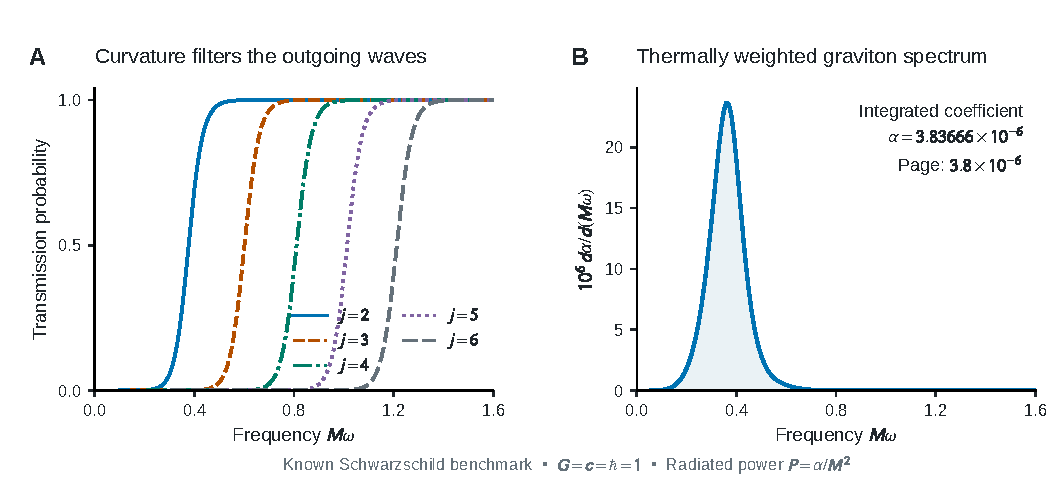
\includegraphics[width=\textwidth]{figs/review_04_graviton_spectrum.pdf}
\caption{\textbf{A known Schwarzschild graviton-emission benchmark.} (A) Regge--Wheeler transmission probabilities for angular momenta $j=2,\ldots,6$. (B) The spectrum after thermal weighting and summation over both helicities. Its shaded integral gives $\alpha=3.83666\times10^{-6}$ and power $P=\alpha/M^2$ in units $G=c=\hbar=1$. The calculation uses 155 frequencies over $0.06\le M\omega\le1.60$ and 2400 radial tortoise-coordinate samples. Page's published total is $3.8\times10^{-6}$~\cite{Page1976}; extra precision of the numerical integral is not extra precision of that reference. The quadrupole supplies $99.06\%$ of the computed power. Agreement tests this scattering calculation, not a derivation of the full quantum theory.}
\label{fig:hawking}
\end{figure*}

\section{Discussion}\label{sec:discussion}

The null-cone construction of Ref.~\cite{Chandrasekaran2026} motivates a finite-resolution model with an explicit occupation budget and finite corner sectors. Proposition~\ref{prop:finite_area} establishes finiteness under these modeling assumptions, without separately postulating a finite list of area sectors. The calculations provide selected classical and semiclassical benchmarks; the Euclidean simulations add evidence for coupling-dependent roughness suppression, now supported by matched controls and a larger-lattice check. Extended local moves improve area sampling at the two tested larger-rank points.

This is not yet a unification of classical general relativity and quantum mechanics. In particular, the full constrained gravitational dynamics, the finite-state Hamiltonian examples, and the sampled Euclidean matrix action have not been shown to define one equivalent theory. The oblate calculation determines primary and secondary brackets on a family of exact bulk trajectories. A physical degree-of-freedom count requires stabilization on the surrounding nonlinear constraint surface and a common radial domain for the canonical generators. Recovery of the gravitational boundary structure and a controlled quantum continuum limit remain open. Agreement with known formulas or identities does not replace those derivations.

Additional dynamical problems remain open:
\begin{enumerate}
\item \emph{Dynamical origin of corner microstates:} In Sec.~\ref{sec:unified}, the discrete embadon corner Hilbert space $\calH_{\mathrm{corner}}(M)$ is specified separately from $I_{\mathrm{G},N}^{\mathrm{bulk}}$. Deriving a discrete area spectrum and its microscopic degeneracy directly from a nonperturbative quantization of $I_{\mathrm{G},N}^{\mathrm{bulk}}$ remains open.
\item \emph{Ultraviolet fixed point at $B\to\infty$:} Fixed-$(s,B)$ projected sums are finite. Establishing whether the full interacting theory with dynamical $\mu^2\to 0$ flows to a non-Gaussian ultraviolet fixed point that tames the two-loop Goroff--Sagnotti growth requires further nonperturbative study.
\item \emph{Emergent Lorentzian horizon shockwaves:} Determining whether microscopic horizon degrees of freedom dynamically reproduce an $\ell$-independent exponential four-dimensional Dray--'t~Hooft Lyapunov shockwave on $S^2$ requires large-local-dimension Schwinger--Dyson ladder kernels or Lorentzian matrix methods beyond small-dimension exact diagonalization, where short-time $O(t^2)$ commutator growth obscures the Lyapunov regime.
\end{enumerate}

To make every step of the audit and regularization independently inspectable, numerical scripts, archived Monte Carlo datasets, and selected logical-dependency and algebraic-identity lemmas in Lean~4.36.0 are cataloged in Appendix~\ref{app:code} and publicly archived.

\begin{acknowledgments}
We warmly thank Venkatesa Chandrasekaran for the classical null-cone reduction, gravitational clock architecture, and Lorentzian axiomatic framework of Ref.~\cite{Chandrasekaran2026}, which motivated this work, and thank independent technical reviewers for incisive comments on the $B(s)=s Q_*$ tail bound, explicit rectangular matrix vertices, the corrected oscillator clock bounds, the modular check on $Z_{\scrD,1}=45$, two-loop finiteness, and effective-field-theory naturalness bounds. We used OpenResearch~\cite{openresearch}, T3 Code, Gemini Neon, and OpenAI GPT-6.2 and GPT-6 Rosalind; simulations ran on a Modal B200 cluster.
\end{acknowledgments}

\appendix

\section{Reconstructed Nonlinear Bulk Action and Separate Matrix Models}\label{app:explicit_action}

\subsection{Why the previous expression must be replaced}

The earlier operator-ordered expression did not pass a bulk variational test even in its commuting spherical sector. Let $X=\rho^2$ and use $h_{ab}dx^a dx^b=-Fdt^2-2Ndt\,dr$. Even after replacing its angular-curvature term by $2N$, the old spherical density, modulo a total derivative, was
\begin{align}
\mathcal L_{\mathrm{old,patch}}&=-2X_r\vartheta+2N-2\Lambda NX,\nonumber\\
\vartheta&=X_t/X-FX_r/(2X).
\end{align}
On $X=r^2$, $N=1$, $F=1-2M/r-\Lambda r^2/3$, its Euler derivatives include $\mathcal E_F=4$ and $\mathcal E_N=2-2\Lambda r^2$, which do not vanish. Boundary terms cannot cancel these residuals for compactly supported variations. Consequently the old expression is withdrawn, as are claims that the archived potential and matrix-product checks verified its first or second variation.

\subsection{A definite nonlinear bulk replacement}

A constructive replacement is an angular Galerkin restriction of the Einstein--Hilbert action. It uses the finite matrices as harmonic coefficient arrays, with ordinary products of their reconstructed functions. It is a different nonlinear prescription from multiplying the matrices inside a normalized trace.

Choose spin-weighted harmonics normalized by $\int |{}_sY_{jm}|^2d\Omega/(4\pi)=1$, with phases matched to the matrix bases. Define
\begin{align}\label{eq:reconstruction_map}
\mathcal R_{s,N}(U)&=\sum_{j=|s|}^{N-1}\sum_{m=-j}^j u_{jm}\,{}_sY_{jm},\nonumber\\
u_{jm}&=\frac{\Tr[(T^{(s,N)}_{jm})^\dagger U]}{\sqrt{N^2-s^2}}.
\end{align}
Use four real spin-zero coefficient arrays for the three components of a symmetric $h_{ab}$ and the angular trace $X$, two complex spin-one arrays for real shifts $A_a^A$, and one complex spin-two array for a real tracefree angular tensor $C_{AB}$. Reality is imposed with the conjugate-spin components. Reconstruct the metric by
\begin{align}\label{eq:galerkin_metric}
ds_N^2&=h_{ab}dx^a dx^b+\gamma_{AB}\Theta^A\Theta^B,\nonumber\\
\Theta^A&=dy^A+A_a^A dx^a,\nonumber\\
\gamma_{AB}&=Xq_{AB}+C_{AB},\qquad q^{AB}C_{AB}=0,
\end{align}
where $q_{AB}$ is the fixed unit-sphere metric and all coefficient fields have the angular cutoff in Eq.~\eqref{eq:reconstruction_map}. Work on the open domain where $h_{ab}$ is Lorentzian and $\gamma_{AB}$ positive definite pointwise. Positivity of a coefficient matrix alone does not establish this domain condition. Away from spherical symmetry, $X$ is half the $q$-trace of $\gamma$, not its area density.

The replacement bulk action is
\begin{equation}\label{eq:explicit_IFSG}
I_{\mathrm{G},N}^{\mathrm{bulk}}[a]
=\frac1{16\pi G_N}\int d^4x\,\sqrt{-g_N[a]}
\big(R[g_N[a]]-2\Lambda\big).
\end{equation}
Here $a$ denotes all retained real coefficient fields, and $R$ is computed using the ordinary Levi-Civita connection. This defines every nonlinear coupling without an ordering ambiguity: reconstruct first, invert and multiply pointwise, differentiate, then integrate the full angular density. Products, inverses, determinants, and the density are not projected back into the retained band. Angular quadrature is a numerical approximation to this integral and must be converged separately.

For compactly supported variations its coefficient equations are exactly
\begin{align}\label{eq:galerkin_eom}
\frac{\delta I_{\mathrm{G},N}^{\mathrm{bulk}}}{\delta a_I(t,r)}
&=-\frac1{16\pi G_N}\int d^2y\sqrt{-g_N}\nonumber\\
&\quad\times(\mathcal G^{\mu\nu}[g_N]+\Lambda g_N^{\mu\nu})
\frac{\partial g^N_{\mu\nu}}{\partial a_I}=0.
\end{align}
Here $\mathcal G^{\mu\nu}[g_N]$ is the Einstein tensor. All ten real metric components are varied; in particular $h_{rr}$ and $A_r^A$ are retained until after variation. A solution of the full Einstein equations that lies in the retained ansatz is stationary for every admissible retained variation. Conversely, vanishing projected equations does not imply vanishing discarded harmonics of the Einstein tensor.

Base-coordinate diffeomorphisms and base-dependent sphere rotations preserve the ansatz. A rotation mixes magnetic indices within each retained multiplet, and its base derivative contributes a degree-one rotational Killing field to the shifts. General angular diffeomorphisms can generate discarded harmonics. The present construction specifies bulk dynamics with compactly supported variations. A causal-diamond variational principle must also pull back a chosen continuum null-boundary and joint action, with its boundary data and normalization of null generators specified~\cite{LehnerEtAl2016}. A quantized boundary algebra and a gluing measure have not been constructed here. Nor has Eq.~\eqref{eq:explicit_IFSG} been identified with the simulated action~\eqref{eq:hmc_action} or the phenomenological vertex~\eqref{eq:cubic_vertex}.

\subsection{Canonical constraints on a stationary oblate solution}

Choose spacelike $t$ slices with $\lambda=h_{rr}>0$. Completing the square in Eq.~\eqref{eq:galerkin_metric} gives the ADM lapse and shift
\begin{align}
\alpha^2&=-h_{tt}+h_{tr}^2/\lambda, &
\beta^r&=h_{tr}/\lambda, &
\beta^A&=A_t^A-\beta^r A_r^A .
\end{align}
The Legendre transform acts on the retained velocities of $(\lambda,X,A_r,C)$. The temporal coefficient fields $z=(h_{tt},h_{tr},A_t)$ have vanishing primary momenta. Their secondary equations are $\delta H/\delta z=0$, with the displayed lapse and shift evaluated pointwise.

\begin{proposition}\label{prop:oblate_rank}
Let $\Lambda=0$, $L=N-1$, and fix a compact radial shell away from the origin. On the static oblate Minkowski family, for sufficiently small nonzero oblateness, the temporal Hamiltonian Hessian has angular rank 18 at $N=3$ and 26 at $N=4$. The Poisson matrix of the combined primary and secondary constraints has local angular rank 36 and 52, respectively, for compactly supported radial tests.
\end{proposition}

\begin{proof}
Write $x=\cos\theta$, $d=1-x^2$, $\rho=r^2+\epsilon$, and $\Sigma=r^2+\epsilon x^2$. The spatial metric is
\begin{equation}
\sigma=\frac{\Sigma}{\rho}dr^2+\frac{\Sigma}{d}dx^2+\rho d\,d\phi^2 .
\end{equation}
The cylindrical radius $\sqrt{\rho d}$ and height $rx$ give the Euclidean metric in these coordinates. Its angular block is $\rho q-\epsilon\,dx\otimes dx$ and $A_r=0$. All coefficient fields have angular degree at most two. With $\alpha=1$, $\beta=0$ the four-metric is an exact stationary vacuum solution in the retained ansatz and its spatial momenta vanish.

For the normalized action $\bar I=(16\pi G_N)/(4\pi)\,I_{\mathrm{G},N}^{\mathrm{bulk}}$, use the spatial DeWitt pairing
\begin{align}
G(U,V)=\frac{1}{4\pi}\int dr\,d^2y\,\sqrt{\det\sigma}\,
\bigl(U_{ij}V^{ij}-\mathrm{tr}_\sigma U\,\mathrm{tr}_\sigma V\bigr).
\end{align}
The restriction of $G$ to the retained spatial tangent space is nondegenerate at the round metric and hence near it. Let $\Pi$ denote its orthogonal tangent projector for this pairing. A shift-coefficient variation $s=(b,W)=(\delta h_{tr},\delta A_t)$ induces $v_s=(b/\lambda)\partial_r+W^A\partial_A$. At fixed zero momentum the spatial velocity absorbs $\Pi\mathcal L_{v_s}\sigma$. The shift Hessian is therefore
\begin{equation}
A(s,t)=-\tfrac12 G(n_s,n_t),\qquad
n_s=(1-\Pi)\mathcal L_{v_s}\sigma .
\end{equation}
The lapse Hessian rows vanish at these data. The terms containing $\partial_r b$ and $\partial_r W$ in the shift Lie derivative are retained spatial variations, so $n_s$ is algebraic in their radial profiles.

Let $V_j$ contain the scalar harmonics through degree $j$. Angular shifts with $W(x)\in V_{L-1}$ and radial shifts with $b/\lambda\in V_{L-2}$ give independent tangent directions. Their dimensions are $2L^2-2$ and $(L-1)^2$, respectively, bounding the rank by $8L+2$. For $m=0,\ldots,L$, exact leading Gram minors of the discarded variations give block ranks $(4,4,3)$ at $L=2$ and $(4,4,4,3)$ at $L=3$. Each positive $m$ contributes twice to the real rank. Analyticity preserves the nonzero minors at sufficiently small nonzero $\epsilon$, giving the matching lower bound and $\ker A=\ker(s\mapsto n_s)$.

The only possible secondary--secondary block pairs a lapse-coefficient test $f$ with a shift test $s$. Its value is $-G(\nabla^2_\sigma f,n_s)/2$ by the flat spatial curvature variation and radial integration by parts. It vanishes on $\ker A$. Eliminating the nondegenerate primary--secondary shift pairs thus gives combined rank $2\,\mathrm{rank}\,A$. Each angular channel still carries a radial function.
\end{proof}

After eliminating the nondegenerate shift pairs, linearized preservation on this family gives one redundant lapse tertiary profile family at $N=3$ and four at $N=4$. For those descriptors the spatial gradient is a retained shift and the tertiary reduces to a shift secondary. The lapse secondaries themselves still apply. The complementary lapse--tertiary brackets have eight and twelve nondegenerate real angular channels, respectively. They are derived with smooth compact radial tests. The reduced bilinear form extends continuously to $H^1_0$ on the shell, where each complementary channel is coercive after a choice of sign. A common boundary domain for the original canonical generators remains to be established.

Higher preservation can exclude data that pass the first two constraint stages. For a round Euclidean slice with $\alpha=1$, $\beta=0$ and constant Cartesian $K_{ij}=\kappa n_i n_j$ ($n$ a unit vector, $\kappa\ne0$), all primaries and secondaries vanish and first preservation admits temporal rates. For every such choice a polar quadrupole shift secondary has nonzero second time derivative for a suitable compact radial test. Thus no sufficiently smooth retained trajectory passes through those fixed data at $N=3,4$. The oblate family tends instead to the round zero-momentum solution. The exact minors, radial forms and second-preservation identity are archived under \path{reports/oblate-constraint-rank-2026-11-27/}, \path{reports/oblate-lapse-consistency-2026-11-27/} and \path{reports/higher-order-consistency-2026-11-27/}, respectively.


\subsection{Spherical reduction and the missing constraint}

For $\gamma_{AB}=Xq_{AB}$ and $A_a^A=0$, exact angular integration and integration by parts give
\begin{align}\label{eq:spherical_repair}
I_{\mathrm{sph}}=\frac1{4G_N}\int d^2x\sqrt{-h}\,
\Big[&XR[h]+\frac{(\nabla X)^2}{2X}\nonumber\\
&+2-2\Lambda X\Big].
\end{align}
Variation precedes null gauge fixing. In the gauge $h_{ab}dx^a dx^b=-Fdt^2-2Ndt\,dr$, $N>0$, one finds
\begin{align}
R[h]&=-\frac1N\partial_r\!\left(\frac{F_r-2N_t}{N}\right),\nonumber\\
\mathcal L_{\mathrm{sph}}&=\frac{X_r(F_r-2N_t)}N-\frac{X_tX_r}X
+\frac{FX_r^2}{2NX}+2N-2\Lambda NX.\label{eq:spherical_density}
\end{align}
The three Euler derivatives of this gauge-fixed density vanish identically on Schwarzschild--de Sitter. They also vanish if $M=M(t)$, exposing why that check alone is insufficient. The covariant metric equation retained by varying first is
\begin{align}
E_{ab}={}&h_{ab}\Box X-\nabla_a\nabla_bX
+\frac{\partial_aX\partial_bX}{2X}\nonumber\\
&-\frac{h_{ab}(\nabla X)^2}{4X}-h_{ab}(1-\Lambda X)=0.
\end{align}
For the time-dependent-mass ansatz $E_{tt}=-2\dot M$; hence vacuum mass conservation is restored. At $N=1$, Eq.~\eqref{eq:spherical_density} agrees with the scalar part of Chandrasekaran's Appendix~B, Eqs.~B.11a--b~\cite{Chandrasekaran2026}.

\subsection{Quadratic sectors and a nonlinear check}

At a spherical Einstein background the first variation of the continuum action vanishes, so the Hessian of its pullback is the continuum Hessian evaluated on the retained linear perturbations. Rotational invariance separates different $j,m$. Because Eq.~\eqref{eq:galerkin_metric} includes all metric components in each retained multiplet, its $j\ge2$ quadratic sectors are the retained Einstein sectors. This is a consequence of the replacement definition, not a property proved for the withdrawn matrix-product action.

An independent symbolic calculation eliminates the constraints in the known Einstein quadratic densities~\cite{Solomon2023}. In the axial sector, with $f=1-2M/r$ and $L=(j-1)(j+2)$,
\begin{equation}
\mathcal L_- =\frac12\left[(\dot h_1-h_0'+2h_0/r)^2
+\frac{Lh_0^2}{r^2f}-\frac{Lf h_1^2}{r^2}\right].
\end{equation}
Its equations give $\dot h_0=f(fh_1)'$ and the Regge--Wheeler equation for $\Psi_-=fh_1/r$. In the polar sector, eliminating the auxiliary field and constraint in Ref.~\cite{Solomon2023}, Eq.~(150), gives the Zerilli potential without inserting it into the starting density. Both symbolic potential residuals vanish for general $j\ge2$.

Map each set of real master harmonics isometrically into $\calB_2^{(N)}$. Define the normalized pairing by
\begin{equation}
\langle U,V\rangle_{2,N}=\frac{\Tr(U^\dagger V)}{\sqrt{N^2-4}}.
\end{equation}
Let $\mathsf L^2$ act with eigenvalue $j(j+1)$. The resulting quadratic action is
\begin{align}\label{eq:quadratic_matrix_action}
I_N^{(2)}=\frac12\sum_{\sigma=\pm}\int dt\,dr_*\Big[&
\|\partial_t\Psi_\sigma\|_{2,N}^2-\|\partial_{r_*}\Psi_\sigma\|_{2,N}^2\nonumber\\
&-\langle\Psi_\sigma,V_\sigma(\mathsf L^2,r)\Psi_\sigma\rangle_{2,N}\Big].
\end{align}
Here $\partial_{r_*}=f\partial_r$, $V_-=f[j(j+1)/r^2-6M/r^3]$, and
\begin{align}
V_+&=\frac{2f\,\mathcal P_\lambda(r)}{r^3(\lambda r+3M)^2},\qquad
\lambda=\frac{(j-1)(j+2)}2,\nonumber\\
\mathcal P_\lambda(r)&=\lambda^2(\lambda+1)r^3+3\lambda^2Mr^2\nonumber\\
&\quad+9\lambda M^2r+9M^3.
\end{align}
The inverse is nonsingular for $j\ge2$ and $r>2M$. Numerical matrix-versus-harmonic bilinear checks at $N=4,6,8$ agree within $5.8\times10^{-12}$.

For a nonlinear check, take $g_N=A(\theta)\bar g_{\mathrm{Schw}}$ with $A=1+\epsilon Y_{20}>0$ and $Y_{20}=\sqrt5P_2(\cos\theta)$. Its metric coefficients fit every $N\ge3$. Direct four-dimensional Ricci evaluation, independent of the conformal-transformation formula, yields the angular-integrated bulk density (with the overall $1/(4G_N)$ suppressed)
\begin{align}
\mathcal L_{\mathrm{ang}}&=\frac32\left\langle\frac{|\nabla_\Omega A|^2}{A}\right\rangle_\Omega\nonumber\\
&=9\epsilon^2-\frac{9\sqrt5}{7}\epsilon^3+O(\epsilon^4).
\end{align}
The exact finite-amplitude integral and its first variation agree with the directly computed Einstein trace at $\epsilon=-0.2,0.1,0.3$. This tests an anisotropic nonlinear family; it is not a general constraint-closure test.

\subsection{Typed matrix maps and the separate gluing example}

For the matrix-product benchmarks, a type-correct scalar action on a spin-$s$ rectangular matrix is
\begin{equation}
F\mathbin{\triangleright_s}U=\tfrac12[\iota_{N\to N+s}(F)U+U\iota_{N\to N-s}(F)].
\end{equation}
It is self-adjoint in the normalized bundle pairing for Hermitian $F$ and sends the identity to the identity, but is not asserted to preserve positivity. Since $\widehat{\bareth}Z\in\calB_1^{(N)}$, its contraction uses $\mathcal S_N^{(1)}$, not $\mathcal S_N^{(2)}$. These fixes make the individual maps well-defined; they do not turn the old action into Eq.~\eqref{eq:explicit_IFSG}.

The following finite gluing Hamiltonian remains a separately specified model, not a canonical quantization of the reconstructed bulk action.


On the 1,260-state spin-$\frac{1}{2}$ multi-sector space $\calH_{\scrD}^{\mathrm{FSG}}=\bigoplus_{M\in\{2,4,6\}}\calH_{\mathrm{corner}}(M)\otimes\calH_{\mathrm{rad}}^{\mathrm{RW+Z}}(M)$ ($s_M=M\ln 2$, $\dim\calH_{\mathrm{corner}}(M)=2^M$, $\dim_{\mathrm{rad}}=15$ spanning $0,1,2$-graviton states of the $j=2$, $k\in\{1,2\}$ Regge--Wheeler and Zerilli cavity modes $\omega_{\mathrm{RW},k},\omega_{\mathrm{Z},k}$), the $SU(2)$-invariant gluing Hamiltonian of Sec.~\ref{sec:unified_H} is
\begin{equation}\label{eq:explicit_HFSG}
H_{\mathrm{glue}} = \hat{s} + \mathbf{1}_{\mathrm{c}}\otimes H_{\mathrm{rad}}^{\mathrm{RW+Z}}
+ g_{\mathrm{glue}}\,\widehat{N}^{-1/2}\,T_{\mathrm{step}}\,\widehat{N}^{-1/2},
\end{equation}
with $g_{\mathrm{glue}}=\frac{1}{4}$, $\hat{s}|_M=(M\ln 2)\mathbf{1}$, $H_{\mathrm{rad}}^{\mathrm{RW+Z}}=\sum_{a=1}^4 \omega_a n_a$, bounded positive inverse lapse $\widehat{N}^{-1}|_M=\mathbf{1}_{\mathrm{c}}\otimes\exp(H_g^{\mathrm{NO}}/s_M)$ constructed from the $C^\infty_c$ focusing kernel $H_g^{\mathrm{NO}}$, and $SU(2)$-intertwining area-stepping operator
\begin{equation}\label{eq:explicit_Tstep}
T_{\mathrm{step}} = \sum_{M\in\{2,4\}}\!\left(V_{\mathrm{c}}^{(M\to M+2)}\otimes V_{\mathrm{r}} + \mathrm{h.c.}\right),
\end{equation}
where $V_{\mathrm{c}}^{(M\to M+2)}:\calH_{\mathrm{corner}}(M)\hookrightarrow\calH_{\mathrm{corner}}(M+2)$ embeds each $(J,m)$ multiplet isometrically into the matching $(J,m)$ multiplicity sector of $M+2$ ($[T_{\mathrm{step}},J_i]=0$), and $V_{\mathrm{r}}=\mathbf{1}_{15}+0.2\sum_{a=1}^4(|1_a\rangle\langle 0|+|0\rangle\langle 1_a|)$ couples the vacuum symmetrically to both Regge--Wheeler and Zerilli single-graviton excitations.


\section{Locations in Chandrasekaran's Manuscript}\label{app:comparison}

The explanations in the main text are self-contained. The following locations in Chandrasekaran's manuscript~\cite{Chandrasekaran2026}, version~1, allow readers to audit the comparison without making its section numbering part of our narrative.

\begin{table*}[t]
\caption{Locations in Chandrasekaran's manuscript~\cite{Chandrasekaran2026} (version~1) and corresponding discussions in this paper. All section, appendix, equation, and axiom numbers in the middle column refer to Chandrasekaran's manuscript; the final column refers to this paper.}
\begin{ruledtabular}
\small
\begin{tabular}{p{0.25\textwidth}p{0.37\textwidth}p{0.29\textwidth}}
Topic & Location in Chandrasekaran (v1) & Treatment in this paper \\
\colrule
Classical null data & Sec.~3; Appendices~A--B & Secs.~\ref{sec:audit_pass}, \ref{sec:unified_action} \\
Open versus closed amplitudes & Eqs.~(4.29), (4.30); (5.30c), (5.38); (5.44), (5.45) & Sec.~\ref{sec:audit_fail}; Eq.~\eqref{eq:trace_gap} \\
Clock domain and vacuum terms & Eqs.~(4.22), (4.27), (5.16), (C.13); Appendix~C.2; vacuum subtraction in Eq.~(D.21) & Secs.~\ref{sec:audit}, \ref{sec:unified_clock} \\
Radiative occupation count & Appendix~D.3 & Sec.~\ref{sec:unified_H} \\
Selected-mode Gaussian amplitude & Sec.~4.4 & Sec.~\ref{sec:orig_44} \\
Entropy coefficients, gluing, backreaction & Secs.~5.3, 5.4, 6 & Secs.~\ref{sec:1loop}, \ref{sec:orig_54}, \ref{sec:orig_6} \\
Conditional algebraic correspondence & Appendix~E.2; finiteness assumption in Axiom~5 & Sec.~\ref{sec:audit_pass}; Appendix~\ref{app:code} \\
\end{tabular}
\end{ruledtabular}
\end{table*}

\ifdefined\ReadingVersion\else\onecolumngrid\fi
\section{Additional Benchmark Figures}\label{app:benchmark_figures}

These figures report selected algebraic, oscillator, and semiclassical tests. Known reference formulas, imposed model parameters, and finite-matrix identities are labeled as such. None of these comparisons constitutes a continuum-limit or equivalence proof.

\begin{figure*}[p]
\centering
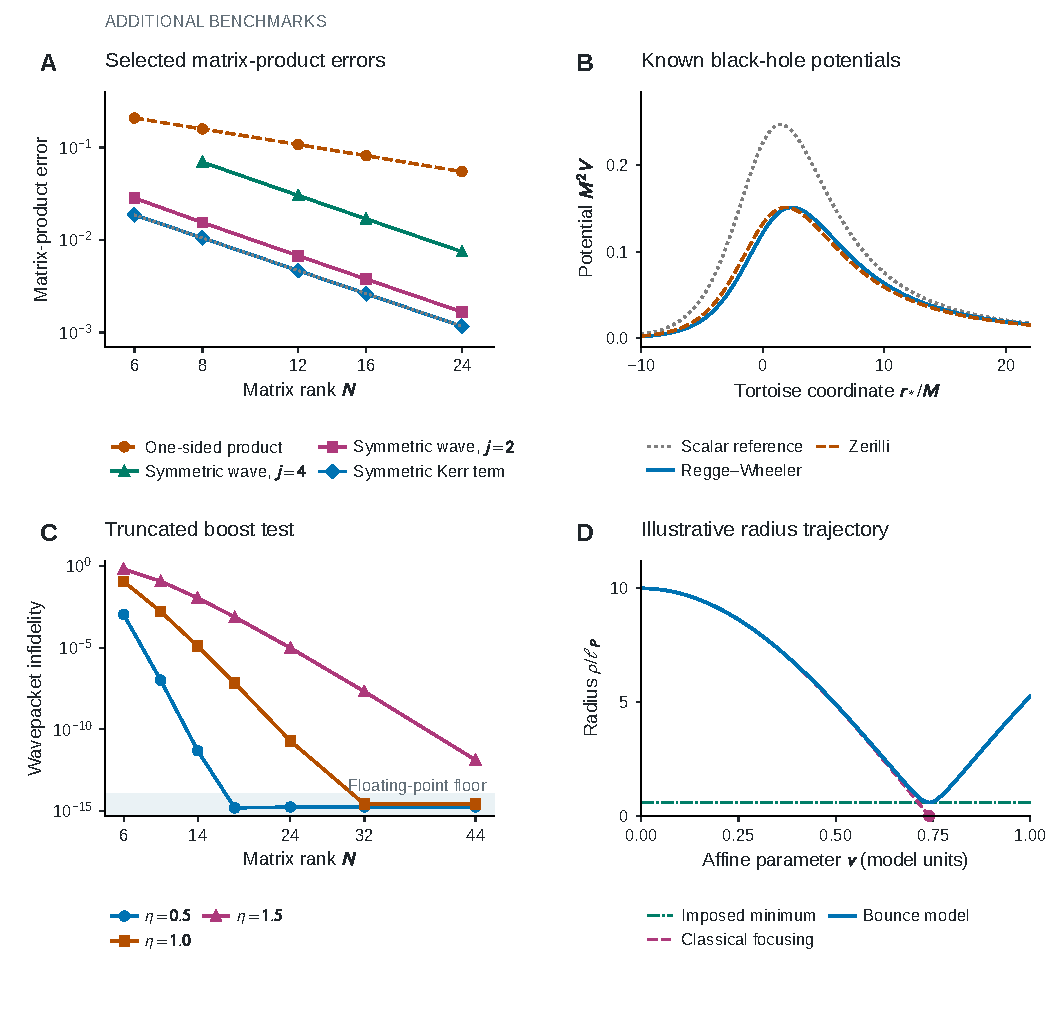
\includegraphics[width=\textwidth]{figs/fig2_unified_matrix_gravity.pdf}
\caption{\textbf{Selected matrix and classical benchmarks.} (A) Errors in chosen Kerr and gravitational-wave matrix products versus continuum coefficients; the symmetric products decrease approximately as $N^{-2}$ over the tested range. (B) Known scalar, Regge--Wheeler, and Zerilli potentials at $j=2$. (C) Infidelity of truncated spin-2 boost wavepackets relative to the reference representation at three rapidities. The shaded range marks values near floating-point precision, not resolved evidence of exact covariance. (D) A classical focusing trajectory compared with an illustrative Ermakov--Pinney trajectory with imposed $\rho_{\min}=\sqrt{\ln3/\pi}\,\lP$. The classical curve stops at its caustic. This example does not derive singularity avoidance from the interacting matrix dynamics.}
\label{fig:unified}
\end{figure*}

\begin{figure*}[p]
\centering
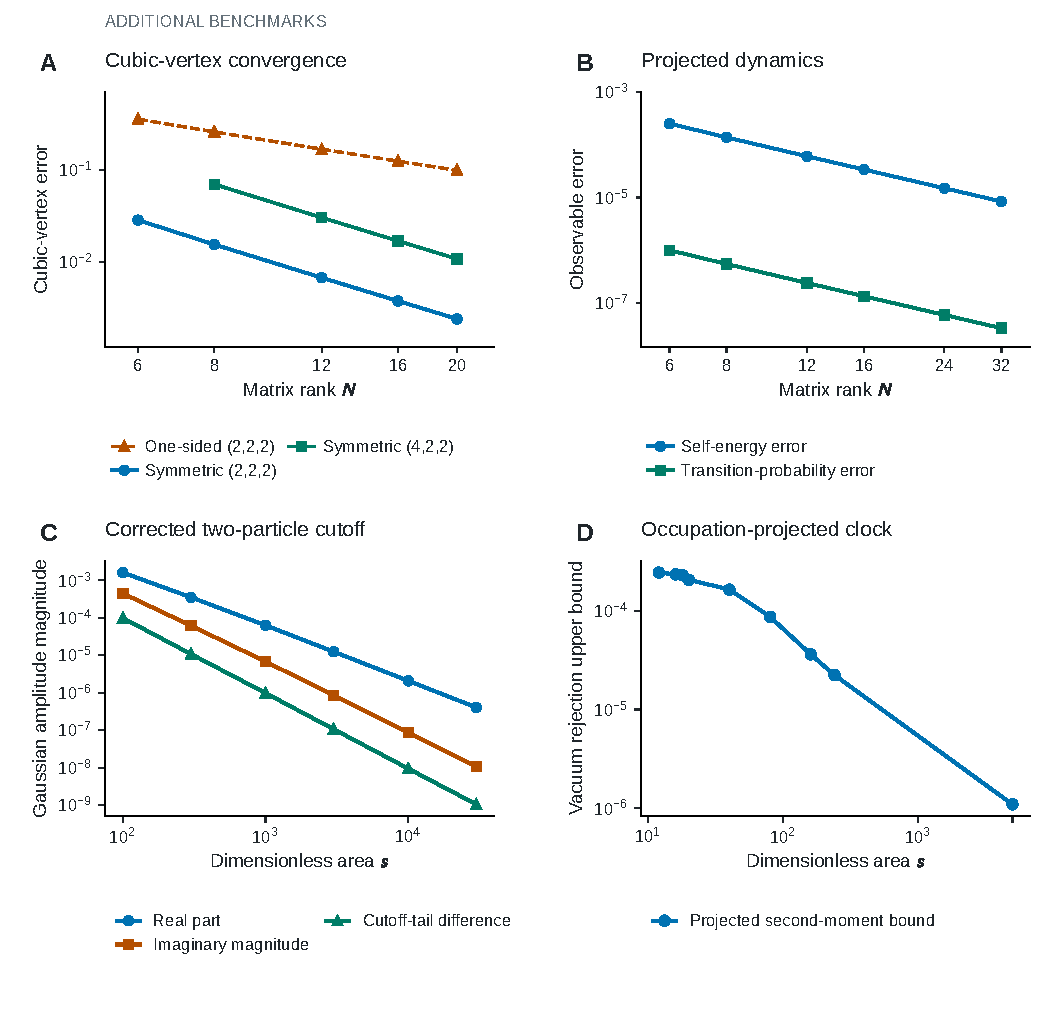
\includegraphics[width=\textwidth]{figs/fig5_v2_unification_and_clock.pdf}
\caption{\textbf{Finite-model vertex, dynamics, amplitude, and clock tests.} (A) Cubic-vertex errors for one-sided and parity-symmetric matrix contractions. (B) Self-energy and transition-probability errors in the finite projected Hamiltonian example relative to its continuum-vertex counterpart. (C) The Gaussian pair sum with the corrected two-particle condition $2\omega_{k,j}\le B(s)=s$; the third curve is its difference from the radial-unrestricted reference. At $B=4$, no pair is allowed. (D) The recomputed second-moment upper bound on vacuum clock-projector rejection for the actual total occupation projector, with $B(s)=0.5s$, $J(s)=\lfloor\sqrt{s/\ln3}\rfloor$, and $\ell/u_{\mathrm{cl}}=2$. The $B=4$ vacuum has exactly zero rejection and is omitted from the logarithmic axis. The old fourth-moment and Chernoff curves do not apply to this compressed exponential and have been removed. Curves are numerical evaluations of bounds, not Monte Carlo observations. These tests have the model scope described in Sec.~\ref{sec:unified}.}
\label{fig:v2}
\end{figure*}

\begin{figure*}[p]
\centering
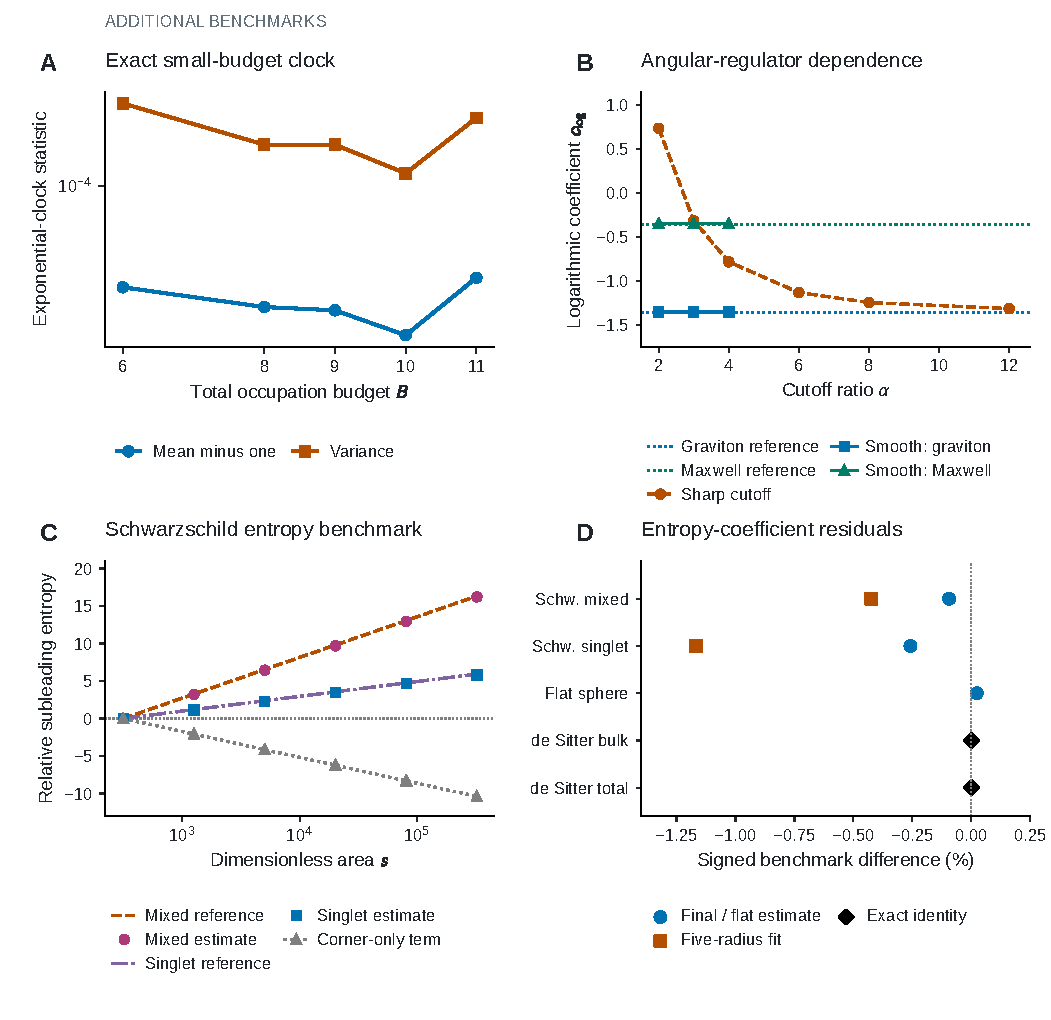
\includegraphics[width=\textwidth]{figs/fig1_breakthrough_1loop.pdf}
\caption{\textbf{Clock and one-loop coefficient benchmarks.} (A) Exact vacuum means and variances of $e^{\Xi_{s,B}}$ for the occupation-projected clock at $s=2B$ and $B<12$. The plotted mean is shown as its excess above one. At $B=4$ both statistics are exactly zero and are omitted from the logarithmic axis. New states entering the budget prevent a monotone interpretation. (B) Extracted flat-space logarithmic coefficients under sharp and smooth angular regulators, compared with known graviton and Maxwell references. (C) Schwarzschild subleading entropy, with a common additive constant removed, compared with the $106/45$ mixed and $77/90$ singlet coefficients. (D) Signed residuals $100(c_{\mathrm{est}}-c_{\mathrm{ref}})/|c_{\mathrm{ref}}|$: final-doubling estimates, five-radius fits, and exact coefficient identities are distinguished by marker. Known heat-kernel inputs and identities make these consistency checks; the plot is not an independent nonperturbative entropy derivation.}
\label{fig:1loop}
\end{figure*}

\begin{figure*}[p]
\centering
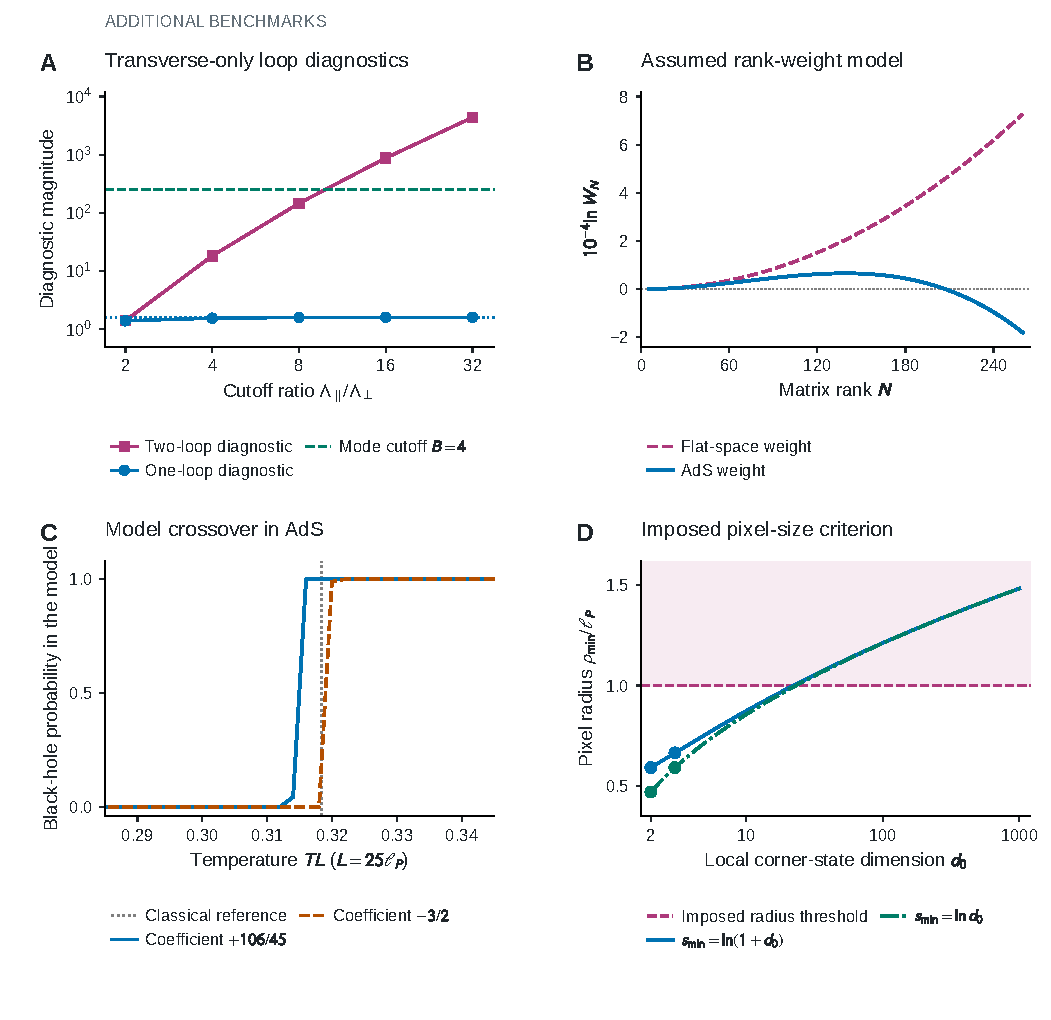
\includegraphics[width=\textwidth]{figs/fig3_uv_completion.pdf}
\caption{\textbf{Regulator and thermodynamic model examples.} (A) Transverse-only loop diagnostics; the horizontal line is the separately regulated single-mode sum at $B=4$. (B) Rank weights computed from the assumed entropy and energy functions for flat space and AdS, with $\beta=L=20$ in Planck units. (C) Black-hole probabilities in the rank-sum model at $L=25\,\lP$, comparing two input logarithmic entropy coefficients; the vertical line is the classical temperature $TL=1/\pi$. (D) Pixel radius as a function of the postulated local corner dimension under two entropy prescriptions. The shaded region violates the imposed radius criterion $\rho_{\min}\le\lP$. These are conditional model calculations, not a derivation of ultraviolet completion or a unique corner spectrum.}
\label{fig:uv}
\end{figure*}

\begin{figure*}[p]
\centering
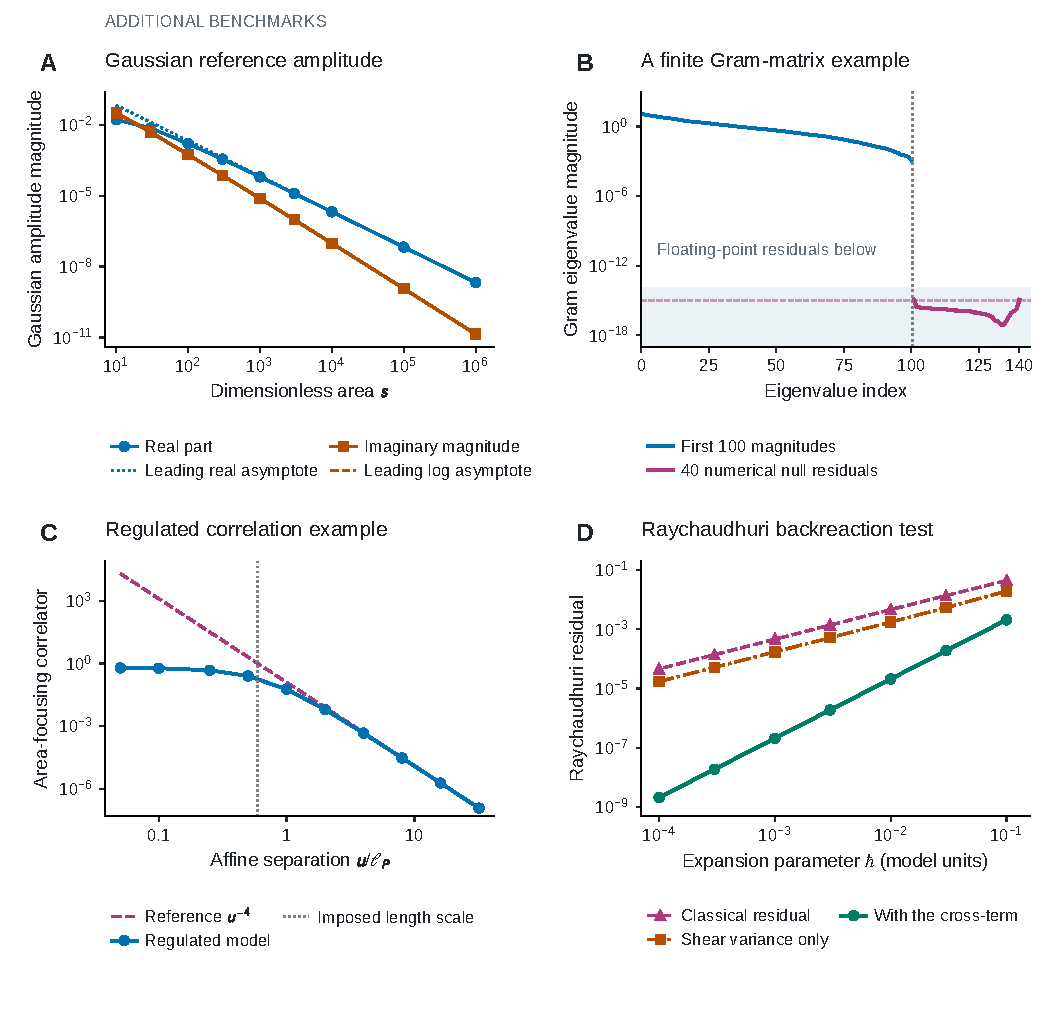
\includegraphics[width=\textwidth]{figs/fig4_original_resolution.pdf}
\caption{\textbf{Gaussian and finite-matrix consistency examples.} (A) A radial-unrestricted Gaussian pair reference with finite angular cutoff, compared with its leading real and imaginary asymptotes. The budget-projected sum is shown separately in Fig.~\ref{fig:v2}(C). (B) Eigenvalue magnitudes of the Gram matrix for 140 constructed fillings in a 100-dimensional operator space. Forty residual magnitudes lie near floating-point precision; the rank bound follows from the chosen algebra. (C) A regulated area-focusing correlator and its large-separation $u^{-4}$ reference. (D) A one-generator Raychaudhuri calculation: retaining the metric--shear cross-term changes the residual scaling from approximately first to second order in the expansion parameter. These examples do not establish a dynamical resolution of topology sums, emergent spacetime, or complete four-dimensional backreaction.}
\label{fig:orig}
\end{figure*}

\clearpage
\ifdefined\ReadingVersion\else\twocolumngrid\fi
\section{Formal Verification Catalog and Code Availability}\label{app:code}

Figure design and evidence-appraisal procedures were informed by Ref.~\cite{ScientificAgentSkills}. All scientific plots and diagrams are generated as editable vector artwork from explicit geometry, equations, or archived numerical inputs. The plotting code records the inputs and distinguishes numerical estimates, illustrative model choices, and known reference expressions.


The repository at \url{https://github.com/ricfulop/fuzzy-null-cone-gravity} contains six Lean modules, symbolic and numerical scripts, Monte Carlo data, and figure sources. The original action-repair and clock checks are in \texttt{verification/repair\_audit\_20261127/}, with equations, provenance, results, and reproduction instructions in \texttt{reports/repair-audit-2026-11-27/}. Legacy scripts and results are retained as historical records; their earlier claims of nonlinear-action variation or a scalar-QEI clock floor are superseded by the present derivations. The archived Lean checks concern the statements encoded in those files. Several statements take the relevant physical or analytic implication as a hypothesis. For example, \texttt{appendix\_E2\_valid\_conditionally} applies an implication supplied in \texttt{SoundRules}; it does not formalize the reconstruction of a Hilbert algebra. The clock incompatibility lemma assumes the growth bound it uses. The archived massive-QEI implications also retain their hypotheses; they do not prove the replacement oscillator inequality in Appendix~\ref{app:clock_proof}. The projection lemma verifies $(1-P)PHP=0$ under algebraic hypotheses, not the identification of $PHP$ with Einstein dynamics. Thus kernel checking certifies these logical and algebraic statements without certifying the full gravitational construction or the Monte Carlo results.

Table~\ref{tab:lean} records the authors' catalog of 50 selected statements. Its scope is conditional implications and exact algebraic or arithmetic identities. The numerical checks are separate and retain their regulator, sampling, and model assumptions.

\begin{table*}[t]
\caption{Catalog of 50 selected Lean statements archived in \texttt{lean4/}.}
\label{tab:lean}
\begin{ruledtabular}
\begin{tabular}{p{0.39\textwidth}cp{0.46\textwidth}}
Lean~4 Module & Theorems & Encoded Logical or Algebraic Scope \\
\colrule
{\footnotesize\texttt{lean4\_verified\_audit.lean}} & 11 & Trace-sum examples; assumed clock growth; conditional E.2 implication \\
{\footnotesize\texttt{lean4\_path2\_breakthrough.lean}} & 9 & Lichnerowicz $+\frac{106}{45}$/$+\frac{77}{90}$, 4D isotropy, conditional QEI, Type~I \\
{\footnotesize\texttt{lean4\_path2\_frontier.lean}} & 8 & Fuzzy monopole $\calB_{s_w}^{(N)}$, $SO(3,1)$ closure, bounce \\
{\footnotesize\texttt{lean4\_path2\_uv\_completion.lean}} & 8 & 2-loop power count, Schw.\ $W^3$, $\mathrm{AdS}_4$, $S_{\mathrm{gen}}$ additivity \\
{\footnotesize\texttt{lean4\_original\_problem\_resolution.lean}} & 7 & Pair-sum asymptotics, $SU(2)$ sectors, backreaction identities \\
{\footnotesize\texttt{lean4\_v2\_reviewer\_fixes.lean}} & 7 & $B(s)$ bounds, $P_B H P_B$, assumed QEI, $Z_{\scrD,1}=45$ mod-8 \\
\colrule
\textbf{Total (zero \texttt{sorryAx}, zero warnings)} & \textbf{50} & Selected logical and algebraic statements \\
\end{tabular}
\end{ruledtabular}
\end{table*}

\section{Uniform Lower Bound for the Specified Quadratic Clock}\label{app:clock_proof}

This appendix proves Eq.~\eqref{eq:clock_floor} for the actual oscillator matrices used in the code. Let $\nu_k=\sqrt{k^2+\mu^2}$, with radial indices $k,l\ge1$. The matrix entries are
\begin{align}
(M_p)_{kl}&=2\sqrt{\nu_k\nu_l}\,(c_{|k-l|}+c_{k+l}),\nonumber\\
(M_q)_{kl}&=\frac{2kl}{\sqrt{\nu_k\nu_l}}(c_{|k-l|}-c_{k+l})
+\frac{2\mu^2}{\sqrt{\nu_k\nu_l}}(c_{|k-l|}+c_{k+l}).
\end{align}
They are positive Gram matrices of sine and cosine functions weighted by $g^2\ge0$. For every finite radial cutoff, the oscillator ground-energy formula and the Powers--St\o rmer inequality~\cite{PowersStormer1970} give
\begin{align}
\inf H_\mu^{\mathrm{NO}}
&=\tfrac12\|\sqrt{M_q}\sqrt{M_p}\|_1-\tfrac14\Tr(M_q+M_p)\nonumber\\
&\ge-\tfrac14\|M_q-M_p\|_1=-\tfrac12\|K_\mu\|_1.
\end{align}
Indeed $\|\sqrt P-\sqrt Q\|_2^2\le\|P-Q\|_1$ and $\|\sqrt P\sqrt Q\|_1\ge\Tr(\sqrt P\sqrt Q)$ for positive $P,Q$. Singular cases follow by adding $\varepsilon\mathbf1$ and taking the finite-dimensional limit.

Put $D=\nu_k\nu_l$. Rationalizing the difference of frequencies gives
\begin{equation}\label{eq:stable_pair_kernel}
(K_\mu)_{kl}=-\frac{\mu^2(k-l)^2c_{|k-l|}}{\sqrt D(D+kl+\mu^2)}
-\frac{D+kl-\mu^2}{\sqrt D}\,c_{k+l}.
\end{equation}
For $l=k+d$, $d\ge1$, the coefficient of $c_d$ is bounded by
$\mu^2d^2/[2(k^2+\mu^2)^{3/2}]$.
The decreasing-function integral comparison gives
$\sum_{k\ge1}\mu^2/(k^2+\mu^2)^{3/2}\le1$ for $\mu>0$; the difference term vanishes at $\mu=0$. Including both triangular halves of the matrix bounds their contribution by $\sum_{d\ge1}d^2|c_d|$.

For the sum term, $0\le(D+kl-\mu^2)/\sqrt D\le k+l$. The upper bound follows from
\begin{align}
&(D+kl-\mu^2)^2-(k+l)^2D\nonumber\\
&\quad=D[2D-k^2-l^2-2\mu^2]-\mu^2(k+l)^2\le0,
\end{align}
using the arithmetic--geometric mean inequality. There are $n-1$ positive pairs $k+l=n$, so its contribution is at most $\sum_{n\ge2}n(n-1)|c_n|$. Bounding trace norm by the sum of absolute entries yields
\begin{equation}
\|K_\mu\|_1\le\sum_{n\ge1}(2n^2-n)|c_n|=2K_g.
\end{equation}
Four integrations by parts give $|c_n|\le C_4/n^4$, where $C_4=\|(g^2)^{(4)}\|_{L^1(0,1)}/(2\pi)^4$. Hence the series converges uniformly in mass and radial cutoff. A finite Fourier sum through $n_0$ can be supplemented with the analytic tail
$C_4[2\zeta(2,n_0+1)-\zeta(3,n_0+1)]$ before division by two. Numerical quadrature of $C_4$ and the finite coefficients is not a certified interval evaluation.

The angular estimate in Proposition~\ref{prop:finite_area} follows from
\begin{equation}
\frac83-\frac{2[(J+1)^2-4]}{J^2}
=\frac{2(J-3)^2}{3J^2}\ge0\qquad(J\ge2).
\end{equation}
Since $\|K\|_2\le\|K\|_1$, each channel contributes at most $2K_g^2$ to the vacuum variance. Compression can only decrease the norm of $\Xi_s|0\rangle$ because $P_B|0\rangle=|0\rangle$. This proves the uniform second-moment bound stated in the main text without a fourth-moment or exponential-integrability assumption. If the clock restriction is imposed on dynamics as well as the state space, its projector must also be included in the Hamiltonian compression; budget preservation alone does not imply clock-sector preservation.


\section{Model Use and Computational Resources}\label{app:model_use}

The documented workflow included extensive steering and seven named hill-climb investigations (H1--H7; 210 model calls), with their usage included in the T3 totals. The supplied OpenResearch and T3 Code usage summaries jointly reported 678 model calls and 151 million processed tokens, including cached prompt reads. Additional ChatGPT/Codex work used GPT-6.2 initially and GPT-6 Rosalind subsequently, across 26 project-related user messages at the accounting cutoff; its token usage was unavailable and is excluded from those totals. Five Modal B200 simulation campaigns comprised 96 production job launches and 565{,}360 chain-level HMC trajectory updates.

The production simulations consumed approximately 4.197 B200 GPU-hours. The trajectory count includes 112{,}560 warm-up updates and 452{,}800 retained updates across chains. Including four reported smoke/operator launches gives approximately 4.27 B200 GPU-hours. These runtime totals exclude billing overhead. No LLM calls were reported inside the Modal simulation jobs.

\begin{thebibliography}{99}

\bibitem{Chandrasekaran2026}
V.~Chandrasekaran, ``An algebraic quantization of gravity from the null cone,'' \href{https://arxiv.org/abs/2611.34924}{arXiv:2611.34924 [hep-th]} (2026).

\bibitem{ChoquetBruhat2011}
Y.~Choquet-Bruhat, P.~T.~Chru\'sciel, and J.~M.~Mart\'in-Garc\'ia, ``The Cauchy problem on a characteristic cone for the Einstein equations in arbitrary dimensions,'' Ann.\ Henri Poincar\'e \textbf{12}, 419 (2011), arXiv:1006.4467.

\bibitem{Reisenberger2008}
M.~P.~Reisenberger, ``The Poisson bracket on free null initial data for gravity,'' Phys.\ Rev.\ Lett.\ \textbf{101}, 211101 (2008), arXiv:0712.2541.

\bibitem{Reisenberger2013}
M.~P.~Reisenberger, ``The symplectic 2-form for gravity in terms of free null initial data,'' Class.\ Quantum Grav.\ \textbf{30}, 155022 (2013), arXiv:1211.3880.

\bibitem{DonnellyFreidel2016}
W.~Donnelly and L.~Freidel, ``Local subsystems in gauge theory and gravity,'' JHEP \textbf{09}, 102 (2016), arXiv:1601.04744.

\bibitem{FreidelGeillerPranzetti2020}
L.~Freidel, M.~Geiller, and D.~Pranzetti, ``Edge modes of gravity. Part II. Corner metric and Lorentz charges,'' JHEP \textbf{11}, 027 (2020), arXiv:2007.03563.

\bibitem{ChandrasekaranFlanagan2023}
V.~Chandrasekaran and \'E.~\'E.~Flanagan, ``Horizon phase spaces in general relativity,'' JHEP \textbf{07}, 017 (2024), arXiv:2309.03871; ``Subregion algebras in classical and quantum gravity,'' arXiv:2601.07915 (2026).

\bibitem{CiambelliFreidelLeigh2024}
L.~Ciambelli, L.~Freidel, and R.~G.~Leigh, ``Null Raychaudhuri: canonical structure and the dressing time,'' JHEP \textbf{01}, 166 (2024), arXiv:2309.03932; ``Quantum null geometry and gravity,'' JHEP \textbf{12}, 028 (2024), arXiv:2407.11132.

\bibitem{CiambelliKlinger2026}
L.~Ciambelli and M.~S.~Klinger, ``Quantization of Gravity on Null Hypersurfaces,'' arXiv:2607.07785 (2026).

\bibitem{CLPW2023}
V.~Chandrasekaran, R.~Longo, G.~Penington, and E.~Witten, ``An algebra of observables for de Sitter space,'' JHEP \textbf{02}, 082 (2023), arXiv:2206.10780.

\bibitem{CPW2023}
V.~Chandrasekaran, G.~Penington, and E.~Witten, ``Large $N$ algebras and generalized entropy,'' JHEP \textbf{04}, 009 (2023), arXiv:2209.10454.

\bibitem{CDMW2024}
E.~Colafranceschi, X.~Dong, D.~Marolf, and Z.~Wang, ``Algebras and Hilbert spaces from gravitational path integrals: Understanding Ryu--Takayanagi/HRT as entropy without AdS/CFT,'' JHEP \textbf{10}, 063 (2024), arXiv:2310.02189.

\bibitem{Sen2013}
A.~Sen, ``Logarithmic Corrections to Schwarzschild and Other Non-extremal Black Hole Entropy in Different Dimensions,'' JHEP \textbf{04}, 156 (2013), arXiv:1205.0971.

\bibitem{MarolfMaxfield2020}
D.~Marolf and H.~Maxfield, ``Transcending the ensemble: baby universes, spacetime wormholes, and the order and disorder of black hole information,'' JHEP \textbf{08}, 044 (2020), arXiv:2002.08950.

\bibitem{Flanagan1997}
\'E.~\'E.~Flanagan, ``Quantum inequalities in two-dimensional Minkowski spacetime,'' Phys.\ Rev.\ D \textbf{56}, 4922 (1997), gr-qc/9706006.

\bibitem{BenedettiCasini2020}
V.~Benedetti and H.~Casini, ``Entanglement entropy of linearized gravitons in a sphere,'' Phys.\ Rev.\ D \textbf{101}, 045004 (2020), arXiv:1908.01800.

\bibitem{ADLS2022}
D.~Anninos, F.~Denef, Y.~T.~A.~Law, and Z.~Sun, ``Quantum de Sitter horizon entropy from quasicanonical bulk, edge, sphere and topological string partition functions,'' JHEP \textbf{01}, 088 (2022), arXiv:2009.12464.

\bibitem{GoroffSagnotti1986}
M.~H.~Goroff and A.~Sagnotti, ``The ultraviolet behavior of Einstein gravity,'' Nucl.\ Phys.\ B \textbf{266}, 709 (1986).

\bibitem{CEMZ2016}
X.~O.~Camanho, J.~D.~Edelstein, J.~Maldacena, and A.~Zhiboedov, ``Causality Constraints on Corrections to the Graviton Three-Point Coupling,'' JHEP \textbf{02}, 020 (2016), arXiv:1407.5597.

\bibitem{HawkingPage1983}
S.~W.~Hawking and D.~N.~Page, ``Thermodynamics of black holes in anti-de Sitter space,'' Commun.\ Math.\ Phys.\ \textbf{87}, 577 (1983).

\bibitem{GrossPerryYaffe1982}
D.~J.~Gross, M.~J.~Perry, and L.~G.~Yaffe, ``Instability of flat space at finite temperature,'' Phys.\ Rev.\ D \textbf{25}, 330 (1982).

\bibitem{KaulMajumdar2000}
R.~K.~Kaul and P.~Majumdar, ``Logarithmic Correction to the Bekenstein--Hawking Entropy,'' Phys.\ Rev.\ Lett.\ \textbf{84}, 5255 (2000), gr-qc/0002040.

\bibitem{Page1976}
D.~N.~Page, ``Particle emission rates from a black hole: Massless particles from an uncharged, nonrotating hole,'' Phys.\ Rev.\ D \textbf{13}, 198 (1976).

\bibitem{BBM2022}
F.~Bastianelli, R.~Bonezzi, and M.~Melis, ``Gauge-invariant coefficients in perturbative quantum gravity,'' Eur.\ Phys.\ J.\ C \textbf{82}, 1139 (2022), arXiv:2206.13287.

\bibitem{FPS2013}
D.~V.~Fursaev, A.~Patrushev, and S.~N.~Solodukhin, ``Distributional geometry of squashed cones,'' Phys.\ Rev.\ D \textbf{88}, 044054 (2013), arXiv:1306.4000.

\bibitem{Steinacker2026}
H.~C.~Steinacker, ``Gravity as a quantum effect on quantum space-time,'' Phys.\ Lett.\ B \textbf{827}, 136946 (2022), arXiv:2110.03936; ``Quantum spacetime and gravity from the IKKT matrix model: an invitation,'' arXiv:2609.08955 (2026).

\bibitem{FewsterEveson1998}
C.~J.~Fewster and S.~P.~Eveson, ``Bounds on negative energy densities in flat spacetime,'' Phys.\ Rev.\ D \textbf{58}, 084010 (1998), gr-qc/9805024.

\bibitem{FewsterFordRoman2010}
C.~J.~Fewster, L.~H.~Ford, and T.~A.~Roman, ``Probability distributions of smeared quantum stress tensors,'' Phys.\ Rev.\ D \textbf{81}, 121901(R) (2010), arXiv:1004.0179.

\bibitem{BalianBrezin1969}
R.~Balian and E.~Br\'ezin, ``Nonunitary Bogoliubov transformations and extension of Wick's theorem,'' Nuovo Cimento B \textbf{64}, 37 (1969).

\bibitem{ScientificAgentSkills}
T.~Kassis, V.~Agarwal, Y.~He, D.~Patel, and A.~M.~Brueckner, ``Scientific Agent Skills: A Library of Procedural Knowledge for Research Agents,'' \href{https://doi.org/10.48550/arXiv.2609.00065}{arXiv:2609.00065} (2026).

\bibitem{openresearch}
alphaXiv, ``OpenResearch: The local-first harness and workspace for research agents'' (2026), \url{https://github.com/alphaXiv/OpenResearch}.

\bibitem{Vehtari2021}
A.~Vehtari, A.~Gelman, D.~Simpson, B.~Carpenter, and P.-C.~B\"urkner, ``Rank-normalization, folding, and localization: An improved $\widehat R$ for assessing convergence of MCMC,'' Bayesian Analysis \textbf{16}, 667--718 (2021), arXiv:1903.08008.

\bibitem{PowersStormer1970}
R.~T.~Powers and E.~St\o rmer, ``Free states of the canonical anticommutation relations,'' Commun.\ Math.\ Phys.\ \textbf{16}, 1--33 (1970), \href{https://doi.org/10.1007/BF01645492}{doi:10.1007/BF01645492}.

\bibitem{Solomon2023}
A.~R.~Solomon, ``Off-Shell Duality Invariance of Schwarzschild Perturbation Theory,'' Particles \textbf{6}, 943--974 (2023), arXiv:2310.04502, \href{https://doi.org/10.3390/particles6040061}{doi:10.3390/particles6040061}.

\bibitem{LehnerEtAl2016}
L.~Lehner, R.~C.~Myers, E.~Poisson, and R.~D.~Sorkin, ``Gravitational action with null boundaries,'' Phys.\ Rev.\ D \textbf{94}, 084046 (2016), arXiv:1609.00207.

\end{thebibliography}

\end{document}
